% - Projeto de pesquisa -
% Apresentação 
% ------------------------------------------------------------------------ 
% ------------------------------------------------------------------------

\documentclass[
	% -- opções da classe memoir --
	12pt,				% tamanho da fonte
	openany,oneside,
%	openright,			% capítulos começam em pág ímpar (insere página vazia caso preciso)
%	twoside,			% para impressão em recto e verso. Oposto a oneside
	a4paper,			% tamanho do papel. 
	% -- opções da classe abntex2 --
	%chapter=TITLE,		% títulos de capítulos convertidos em letras maiúsculas
	%section=TITLE,		% títulos de seções convertidos em letras maiúsculas
	%subsection=TITLE,	% títulos de subseções convertidos em letras maiúsculas
	%subsubsection=TITLE,% títulos de subsubseções convertidos em letras maiúsculas
	% -- opções do pacote babel --
	english,			% idioma adicional para hifenização
	brazil,				% o último idioma é o principal do documento
	]{abntex2}

% ---
% PACOTES
% ---

% ---
% Pacotes fundamentais 
% ---
\usepackage{lmodern}			% Usa a fonte Latin Modern
\usepackage[T1]{fontenc}		% Selecao de codigos de fonte.
\usepackage[utf8]{inputenc}		% Codificacao do documento (conversão automática dos acentos)
\usepackage{indentfirst}		% Indenta o primeiro parágrafo de cada seção.
\usepackage{color}				% Controle das cores
\usepackage{graphicx}			% Inclusão de gráficos
\usepackage{microtype} 			% para melhorias de justificação

\DeclareUnicodeCharacter{2212}{\textendash}

% ---

% ---
% Pacotes adicionais, usados apenas no âmbito do Modelo Canônico do abnteX2
% ---
\usepackage{lipsum}				% para geração de dummy text
% ---

% ---
% Pacotes de citações
% ---
\usepackage[brazilian,hyperpageref]{backref}	 % Paginas com as citações na bibl
\usepackage[alf]{abntex2cite}	% Citações padrão ABNT

\usepackage{soul}
\usepackage{amsmath}
\usepackage[table]{xcolor}
\usepackage{multicol}
\usepackage{tikz}
\usepackage{pgfgantt}
\usepackage{enumitem}


% --- 
% CONFIGURAÇÕES DE PACOTES
% --- 

% ---
% Configurações do pacote backref
% Usado sem a opção hyperpageref de backref
\renewcommand{\backrefpagesname}{Citado na(s) página(s):~}
% Texto padrão antes do número das páginas
\renewcommand{\backref}{}
% Define os textos da citação
\renewcommand*{\backrefalt}[4]{
	\ifcase #1 %
		Nenhuma citação no texto.%
	\or
		Citado na página #2.%
	\else
		Citado #1 vezes nas páginas #2.%
	\fi}%
% ---

% ---
% Informações de dados para CAPA e FOLHA DE ROSTO
% ---
\titulo{A complexidade estatística em redes de aprendizagem profunda como critério de escolha e otimização em problemas de imagens médicas}
\autor{Luiz Otavio Murta Junior}
\local{Ribeirão Preto/SP}
\data{2022, v<VERSION>}
\instituicao{%
  Universidade de São Paulo -- USP
  \par
  Faculdade de Filosofia, Ciências e Letras de Ribeirão Preto
  \par
  Departamento de Computação e Matemática}
\tipotrabalho{Projeto de Pesquisa FAPESP}
% O preambulo deve conter o tipo do trabalho, o objetivo, 
% o nome da instituição e a área de concentração 
\preambulo{Modelo canônico de Projeto de pesquisa em conformidade
com as normas ABNT apresentado à comunidade de usuários \LaTeX.}
% ---

% ---
% Configurações de aparência do PDF final

% alterando                                                                                                                                                                                                                                                                                               o aspecto da cor azul
\definecolor{blue}{RGB}{41,5,195}

% informações do PDF
\makeatletter
\hypersetup{
     	%pagebackref=true,
		pdftitle={\@title}, 
		pdfauthor={\@author},
    	pdfsubject={\imprimirpreambulo},
	    pdfcreator={LaTeX with abnTeX2},
		pdfkeywords={abnt}{latex}{abntex}{abntex2}{projeto de pesquisa}, 
		colorlinks=true,       		% false: boxed links; true: colored links
    	linkcolor=blue,          	% color of internal links
    	citecolor=blue,        		% color of links to bibliography
    	filecolor=magenta,      		% color of file links
		urlcolor=blue,
		bookmarksdepth=4
}
\makeatother
% --- 

% --- 
% Espaçamentos entre linhas e parágrafos 
% --- 

% O tamanho do parágrafo é dado por:
\setlength{\parindent}{1.3cm}

% Controle do espaçamento entre um parágrafo e outro:
\setlength{\parskip}{0.2cm}  % tente também \onelineskip

\setlrmarginsandblock{3cm}{1.5cm}{*}
\setulmarginsandblock{3cm}{1.5cm}{*}
\checkandfixthelayout


%\renewcommand{\thesection}{\arabic{section}}

% ---
% compila o indice
% ---
\makeindex
% ---

% ----
% Início do documento
% ----
\begin{document}

% Seleciona o idioma do documento (conforme pacotes do babel)
%\selectlanguage{english}
\selectlanguage{brazil}

% Retira espaço extra obsoleto entre as frases.
\frenchspacing 

% ----------------------------------------------------------
% ELEMENTOS PRÉ-TEXTUAIS
% ----------------------------------------------------------
% \pretextual

% ---
% Capa
% ---
%\imprimircapa
% ---

% ---
% Folha de rosto
% ---
%\imprimirfolhaderosto
% ---

% ---
% NOTA DA ABNT NBR 15287:2011, p. 4:
%  ``Se exigido pela entidade, apresentar os dados curriculares do autor em
%     folha ou página distinta após a folha de rosto.''
% ---
\begin{center}
\textbf{\centering\Large A complexidade estatística em redes de aprendizagem profunda como critério de escolha e otimização em problemas de imagens médicas}
\end{center}

\begin{tabular}{c@{\hskip 2cm}c}
Pesquisador Principal: & Luiz Otavio Murta Junior
\end{tabular}

\setlength{\absparsep}{12pt} % ajusta o espaçamento dos parágrafos do resumo
\begin{resumo}
Desde o seu renascimento, o aprendizado profundo (deep learning - DL) tem sido amplamente utilizado em várias tarefas de imagens médicas e alcançou um sucesso notável em muitas aplicações de imagens médicas, impulsionando-nos assim para a chamada era da inteligência artificial (IA). 
Sabe-se que o sucesso da IA é atribuído principalmente à disponibilidade de grandes conjuntos de dados (big data) com anotações para uma única tarefa e aos avanços na computação de alto desempenho. No entanto, a imagem médica apresenta desafios únicos que confrontam as abordagens de DL e possuem evoluções estruturais e dinâmicas em seus modelos ainda pouco conhecidos. 
Neste projeto de pesquisa, vislumbra-se validar um instrumento para o estudo de melhores arquiteturas de rede, bem como a análise de evolução estrutural e dinâmicas para diferentes problemas em imagens médicas. As aplicações a serem estudadas serão segmentação e apoio ao diagnóstico por imagens médicas por DL baseada em imagens. A ferramenta matemática e estatística proposta para a estimativa da complexidade estatística a ser aferida sobre o padrão de pesos da rede será a complexidade \texttt{LMC}. A complexidade estatística \texttt{LMC} é estimada como o produto da entropia de Shannon pela distância estatística do equilíbrio será testada e validada como uma métrica de auto-organização da rede enquanto comparada com a eficiência do DL. Além disso, as ferramentas de análises dinâmica e estrutural que também serão investigadas são respectivamente entropia amostral (\texttt{SampEn}), entropia amostral bidimensional (\texttt{SampEn\textsubscript{2D}}), bem como suas aferições em multiplas escalas (multiscale entropy – \texttt{MSE}) como estimativas de irregularidade estrutural. Com este estudo se pretende entender melhor o que ocorre internamente na rede durante o DL enquanto lida com imagens médicas e quais as melhores arquiteturas de redes profundas em aplicações específicas.

\textbf{Palavras-chaves:} Imagens médicas; Inteligência artificial; Aprendizagem profunda; irregularidade estrutural; Complexidade estatística; Suporte ao diagnóstico; Segmentação de imagens.

\textbf{\centering\large Departamento de Computação e Matemática\\
					Faculdade de Filosofia, Ciências e Letras de Ribeirão Preto - USP}

\end{resumo}
%\clearpage

\begin{center}
\textbf{\centering\Large The statistical complexity of deep learning networks as choice and optimization criteria in medical imaging problems}
\end{center}

\begin{tabular}{c@{\hskip 2cm}c}
Principal Investigator: & Luiz Otavio Murta Junior 
\end{tabular}

\setlength{\absparsep}{12pt} % ajusta o espaçamento dos parágrafos do resumo
\begin{resumo}[Abstract]
 \begin{otherlanguage*}{english}
Since its renaissance, deep learning (DL) has been widely used in various medical imaging tasks and has achieved remarkable success in many medical imaging applications, thereby propelling us into the so-called artificial intelligence (AI) era. The success of AI is well known and mainly attributed to the availability of big data with annotations for a single task and the advances in high-performance computing. However, medical imaging presents unique challenges that confront DL approaches and have structural and dynamic evolutions in their models that are still little known. This research project envisaged the study and validation of a tool for the choice of better network architectures and the analysis of structural and dynamic evolution for different problems in medical imaging. The applications to be studied will be segmentation and support for medical imaging diagnosis based on DL. The proposed mathematical and statistical tool to estimate the statistical complexity of the network weights pattern will be measured by the \texttt{LMC} complexity. The \texttt{LMC} statistical complexity estimated as the product of Shannon entropy by the statistical distance from equilibrium, i.e., disequilibrium, will be tested and validated as a metric of self-organization of the network while comparing to DL efficiency. In addition, we will investigate sample entropy (\texttt{SampEn}), two-dimensional sample entropy (\texttt{SampEn\textsubscript{2D}}), and their multiscale versions (\texttt{MSE}) as the dynamic and structural analysis tools of deep network units during DL training. With this study, we intend to understand better what happens inside the network during DL while dealing with medical images and the best deep network architectures in specific applications.

\textbf{Keywords: }Medical images; Artificial intelligence; Deep learning; Structural irregularity; Statistical complexity; Diagnostic support; Image segmentation; Image-guided therapy.

\textbf{\centering\large Department of Computing and Mathematics \\
					Faculty of Philosophy, Sciences and Letters of Ribeirão Preto - USP}
 \end{otherlanguage*}
\end{resumo}
\clearpage







% ---
% inserir lista de ilustrações
% ---
%\pdfbookmark[0]{\listfigurename}{lof}
%\listoffigures*
%\cleardoublepage
% ---

% ---
% inserir lista de tabelas
% ---
%\pdfbookmark[0]{\listtablename}{lot}
%\listoftables*
%\cleardoublepage
% ---

% ---
% inserir lista de abreviaturas e siglas
% ---
%\begin{siglas}
%  \item[ABNT] Associação Brasileira de Normas Técnicas
%  \item[abnTeX] ABsurdas Normas para TeX
%\end{siglas}
% ---

% ---
% inserir lista de símbolos
% ---
%\begin{simbolos}
%  \item[$ \Gamma $] Letra grega Gama
%  \item[$ \Lambda $] Lambda
%  \item[$ \zeta $] Letra grega minúscula zeta
%  \item[$ \in $] Pertence
%\end{simbolos}
% ---

% ---
% inserir o sumario
% ---
\pdfbookmark[0]{\contentsname}{toc}
\tableofcontents*
\cleardoublepage
% ---


% ----------------------------------------------------------
% ELEMENTOS TEXTUAIS
% ----------------------------------------------------------
\textual
\setcounter{page}{1}

% ----------------------------------------------------------
% Introdução
% ----------------------------------------------------------
\chapter{Introdução}
%\section*{1 Introdução}
%\addcontentsline{toc}{chapter}{Introdução}

O presente projeto tem por objetivo propor e avaliar a complexidade de diferentes arquiteturas de redes DL (do inglês, \textit{deep learning}), ou redes profundas, para diferentes aplicações de imagens médicas, observando a complexidade dinâmica e estrutural das redes durante o seu aprendizado. No contexto das arquiteturas, se sabe que as redes profundas DL possuem uma variedade de tipos, passando por camadas de redes convolucionais CNN (do inglês, \textit{convolutional neural network}), camadas de redução de dimensionalidade (\textit{max-pooling}), camadas densas (totalmente conectada), entre outras. Nestes termos, podemos investigar a complexidade ou irregularidade dinâmica e estrutural que é adquirida pela rede ao resolver problemas de imagens médicas.

A imagem médica explora fenômenos físicos, como luz, radiação eletromagnética, radioatividade, ressonância magnética nuclear (RM) e som para gerar representações visuais ou imagens de tecidos externos ou internos do corpo humano, ou de uma parte do corpo humano, de forma não invasiva, ou por meio de um procedimento invasivo \cite{c1}. As modalidades de imagem mais comumente usadas na medicina clínica incluem radiografia de raios-X, tomografia computadorizada (TC), imagem de ressonância magnética (MRI), ultrassom e patologia digital. Os dados de imagem representam cerca de 90\% de todos os dados de saúde, e portanto, são uma das fontes de evidência mais importantes para análises clínicas e intervenções médicas.

A DL foi considerada uma das dez tecnologias inovadoras de 2013 \cite{c3}. Isso se seguiu ao desafio de categorização de imagens em grande escala de 2012, que introduziu a superioridade da CNN no conjunto de dados ImageNet \cite{c4}. Naquela época, o DL emergiu como a principal ferramenta de aprendizado de máquina nos domínios de imagem geral e visão computacional, e a comunidade de imagens médicas começou um debate sobre se o DL seria aplicável no espaço de imagens médicas. As preocupações eram devidas aos desafios descritos acima, sendo o principal desafio a falta de dados rotulados suficientes, conhecido como desafio dos dados. Várias etapas podem ser apontadas como facilitadores da tecnologia de DL no espaço de imagens médicas: em 2015-2016, as técnicas foram desenvolvidas usando transferência de aprendizagem (Transfer Learning - TL), ou o que também foi chamado de "aprendizagem de recursos não médicos" \cite{c5} para aplicar o conhecimento obtido através da resolução de um problema de origem a um problema de destino diferente, mas relacionado. Uma questão chave era se uma rede pré-treinada em imagens naturais seria aplicável a imagens médicas. Vários grupos mostraram ser este o caso \cite{c6,c7}; usar a rede profunda treinada com base em ImageNet e fazer o ajuste fino em uma tarefa de imagem médica foi útil para acelerar a convergência de treinamento e melhorar a precisão.

Ferramentas de inteligência artificial (IA), como a tecnologia DL, podem fornecer suporte aos médicos automatizando a análise de imagens, levando ao que podemos chamar de radiologia computacional. As ferramentas automatizadas que podem ser desenvolvidas são detecção de achados patológicos, quantificação da extensão da doença, caracterização de patologias (por exemplo, em benigna versus maligna) e ferramentas de software variadas que podem ser amplamente caracterizadas como suporte à decisão. Esta tecnologia também pode estender as capacidades dos médicos para incluir a caracterização de eventos tridimensionais e variáveis no tempo, que muitas vezes não são incluídos nos relatórios radiológicos de hoje devido ao tempo limitado e às ferramentas de visualização e quantificação limitadas. 



\section{Problemas no uso da IA com imagens médicas}

A imagem médica tem várias características que influenciam a adequação e a natureza das soluções de aprendizado profundo (DL). Observe que esses traços não são necessariamente exclusivos da imagem médica. Por exemplo, imagens de satélite compartilham a primeira característica descrita a seguir com imagens médicas. As imagens médicas têm múltiplas modalidades e são densas na sua resolução de pixels, além de já ter muitas modalidades, novas modalidades, como TC espectral, são inventadas rotineiramente. Mesmo para modalidades de imagem comumente usadas, a resolução de pixel ou voxel aumentou, aumentando a densidade da informação. 

Por exemplo, a resolução espacial da tomografia e ressonância magnética clínica atingiu o nível submilimétrico, enquanto os tomógrafos de hoje podem adquirir 1000–2500 cortes por indivíduo, a resolução espacial do ultrassom é ainda melhor, enquanto sua resolução temporal ultrapassa o tempo real. Como resultado, uma única imagem de patologia digital em lâmina correspondente a um único núcleo de biópsia da próstata pode facilmente ocupar 10 GB de espaço com uma ampliação de 40 vezes. No geral, bilhões de estudos de imagens médicas são realizados por ano em todo o mundo, e esse número está crescendo. 

Os rótulos associados às imagens médicas são esparsos e ruidosos. Rotular ou anotar uma imagem médica é demorado e caro. Além disso, diferentes tarefas requerem diferentes formas de anotação, o que cria o fenômeno da dispersão do rótulo. Devido à experiência e às condições variáveis, as inconsistências de rotulagem entre usuários e intrausuários são altas \cite{c2}, e os rótulos devem ser considerados ruidosos. O estabelecimento de padrões ouro para a rotulagem de imagens permanece uma questão em aberto.

Em 2017-2018, o aumento de dados sintéticos surgiu como uma segunda solução para processar conjuntos de dados limitados. Obviamente, o aumento clássico é um componente vital de qualquer treinamento de rede. Ainda assim, as principais questões a serem abordadas eram se era possível sintetizar dados médicos usando esquemas, como modelagem generativa, e se os dados sintetizados serviriam como exemplos médicos viáveis e iriam, na prática, aumentar o desempenho da tarefa médica em questão. Vários trabalhos em vários domínios demonstraram que esse era, de fato, o caso. 
Por exemplo, em \cite{c8}, o aumento da imagem sintética com base na rede adversária geradora (GAN) mostrou gerar amostras de imagem da lesão que não foram reconhecidas como sintéticas pelos radiologistas especialistas e aumentou o desempenho da CNN na classificação de lesões hepáticas. GANs, codificadores variacionais e variações ainda estão sendo explorados e avançados em trabalhos recentes.

Uma das contribuições críticas que emergiram da comunidade de imagens médicas para segmentação de imagens foi a arquitetura U-Net \cite{c9}. Projetada inicialmente para segmentação de células microscópicas, a U-Net provou aprender recursos práticos de forma eficiente e robusta para muitas tarefas de segmentação de imagens médicas.

\section{Redes de Aprendizado Profundo (DL)}
As redes neurais profundas têm uma capacidade de modelo maior e uma capacidade de generalização mais robusta do que as redes neurais superficiais. Modelos profundos treinados em bancos de dados anotados em grande escala para uma única tarefa alcançam desempenhos excepcionais, muito além dos algoritmos tradicionais ou mesmo da capacidade humana. A partir do AlexNet \cite{c4}, houve uma tendência de pesquisa para aprofundar as redes, como representado por VGGNet \cite{c10}, Inception Net \cite{c11} e ResNet \cite{c12}. Conexões de salto tornam uma rede profunda mais treinável do que DenseNet \cite{c13} e U-Net \cite{c9}. A U-net foi proposta pela primeira vez para lidar com a segmentação, enquanto as outras redes foram desenvolvidas para a classificação de imagens. A supervisão profunda \cite{c14} melhora ainda mais o poder discriminativo.

Mecanismos de atenção adversários (GAN) Goodfellow et al. \cite{c15} propõem acompanhar um modelo gerador com um discriminador que diz se uma amostra é da distribuição do modelo ou da distribuição de dados. Redes profundas representam o gerador e o discriminador, e seu treinamento é feito por meio de uma otimização minimax. A aprendizagem adversária é amplamente usada em imagens médicas \cite{c16}, incluindo reconstrução de imagens médicas \cite{c17}, aprimoramento da qualidade de imagem \cite{c18} e segmentação \cite{c19}. O mecanismo de atenção \cite{c20} permite a descoberta automática de “onde” e “o que” focar ao descrever o conteúdo da imagem ou tomar uma decisão holística. O aperto e a excitação \cite{c21} podem ser considerados um canal de mecanismo de atenção. Atenção é combinada com GAN em \cite{c22} e com U-Net em \cite{c23}.

Pesquisa de arquitetura neural (NAS) e design leve: NAS \cite{c24} tem como objetivo projetar automaticamente uma arquitetura de rede profunda para alto desempenho voltada para uma determinada tarefa. Zhu et al. \cite{c25} aplicar NAS com sucesso à segmentação volumétrica de imagens médicas. Por outro lado, o design leve \cite{c26, c27}, por outro lado, visa projetar a arquitetura para eficiência computacional em dispositivos com recursos limitados, como telefones celulares, mantendo a precisão. Para lidar com rótulos esparsos e barulhentos, precisamos de abordagens DL que sejam eficientes em relação a anotações. Assim, a ideia principal é aproveitar o poder e a robustez da capacidade de representação de recursos derivada de modelos e dados existentes, mesmo que os modelos ou dados não sejam necessariamente do mesmo domínio ou para a mesma tarefa, e se adaptar.



\section{Complexidade}
O conceito de complexidade estatística decorre da teoria do caos onde, para vários sistemas não lineares existe transição entre regime ordenado, regular, e não caótico para o regime caótico, onde a aleatoriedade absoluta rege o sistema. A complexidade estatística LMC conforme definida mais adiante mais cuidadosamente é composta como o produto entre a entropia de Shannon e a distância do equilíbrio, ou desequilíbrio \cite{c28}. A complexidade estatística inspira o conceito de complexidade fisiológica, através do qual Goldberger et. al., \cite{c29, c30, c31} relacionam a complexidade ao bom funcionamento dos sistemas fisiológicos autorregulados, o que permite várias funções essenciais à vida. Além disso, os trabalhos de Goldberger et. al., associam os mecanismos de doença e envelhecimento de sistemas fisiológicos com a queda de complexidade. Portanto, a complexidade estaria ligada à capacidade dos seres vivos de se adaptarem às várias situações encontradas, por outro lado, a baixa complexidade estaria relacionada às condições patológicas e envelhecimento com a falta de eficiência e adaptabilidade.

A situação de auto-organização e complexidade somente existe na região chamada de borda do caos (edge of chaos), exatamente onde se observa espaços com dimensões fractais que parece permitir a emergência de comportamentos interessantes e intrigantemente ligados à possibilidade de existência da vida. \textbf{A hipótese central aqui é a de que a complexidade em IA deep learning ou deep network está relacionada diretamente à eficiência e capacidade de adaptação, ou adaptabilidade, das redes.}

A entropia amostral \texttt{SampEn} (do inglês, \textit{sample entropy}) e a entropia multiescala \texttt{MSE} (do inglês, \textit{multiscale entropy}) fornecem insights sobre a complexidade das flutuações ao longo de uma gama de escalas de tempo e é uma extensão das medidas de entropia de amostra padrão descritas aqui \cite{c32,c31}. Como qualquer medida de taxas de entropia, o objetivo é fazer uma avaliação da complexidade de uma série temporal. Uma das principais razões para usar uma abordagem multiescala é quando a escala de tempo de relevância na série temporal não é conhecida. Por exemplo, se olharmos para a fala, seria relevante considerar as escalas de tempo das palavras em vez de sons individuais, mas se você não tinha nenhuma ideia de que o sinal de áudio representava a fala, ou talvez mesmo qualquer ideia do conceito de fala, você não saberia qual escala de tempo seria mais informativa. Portanto, seria mais informativo olhar para um intervalo de escalas de tempo. No sinais fisiológicos, o código subjacente é desconhecido e, portanto, a escala de tempo de relevância é desconhecida \cite{c33, c34}. Recentemente, tem sido proposto e aplicado em diferentes situações a entropia multiescala bidimensional \texttt{MSE\textsubscript{2D}} para medir e analisar a irregularidade e complexidade de texturas em imagens \cite{c35}.

\chapter{Objeto de pesquisa}
Diante do exposto, o presente projeto se distingue por avançar por além das avaliações das aplicações, analisando a evolução da complexidade estrutural e dinâmica de rede durante o DL nestas diferentes aplicações. Entende-se por complexidade estrutural, no contexto de redes DL, o nível mensurável de auto-organização dos padrões de pesos sinápticos adquiridos durante o treinamento.

A hipótese que se pretende investigar é a de que as redes profundas convergem para um estado de auto-organização dos padrões de pesos (sinápticos) durante o processo de aprendizado supervisionado. 

A complexidade pode ser vista como forma de medir o grau de auto-organização da rede DL, pode qualificar o treinamento, permitindo a escolha de diferentes técnicas de aprendizado DL e arquiteturas de rede adequadas a diferentes aplicações em imagens médicas. Cabe ressaltar que é previsto que a tendência de ganho de complexidade durante o aprendizado seja maior quando tratamos de imagens médicas comparativamente ao tratamento de imagens ordinárias como fotografia. Este aspecto comparativo entre imagens fotográficas ordinárias e imagens médicas em diferentes modalidades será um dos pontos do estudo dentre as diferentes investigações possíveis neste contexto.

\chapter{Materiais e Métodos}
O presente projeto pretende estudar a complexidade intrínseca de redes DL usando as linguagens \texttt{python} e \texttt{C++}, apresentando para as redes DL imagens médicas de diferentes modalidades, utilizando as ferramentas TensorFlow e pyTorch para a construção das redes e treinamento. As diferentes arquiteturas que serão testadas em diferentes conjuntos de modalidades diferentes de imagens médicas com a finalidade de mensurar a qualidade da rede DL e do treinamento através das medidas aqui colocadas, i.e., a \texttt{LMC} e a \texttt{SampEn}.

O TensorFlow é um sistema de aprendizado de máquina que opera em larga escala e em ambientes heterogêneos. O TF usa grafos de fluxo de dados para representar a diferentes etapas de computação, os estados compartilhados e as operações que alteram esse estado. Ele mapeia os nós de um grafo de fluxo de dados em muitas máquinas em um cluster e em uma máquina em vários dispositivos computacionais, incluindo unidades centrais de processamento (central processicing units – CPUs) de múltiplos núcleos, unidades gráficas de processamento (graphic processing units – GPUs) de propósito geral (GPGPUs) e unidades  de processamento de tensores (tensor processing units - TPUs) \cite{c36}. Essa arquitetura oferece flexibilidade no desenvolvimento de aplicações, avaliações e pesquisas na área de aprendizado de máquina e inteligência artificial, o TF permite o desenvolvimento experimental de novas otimizações e algoritmos de treinamento. O TF é compatível com uma variedade de aplicativos, com foco no treinamento e inferência em redes neurais profundas. Vários serviços do Google usam o TF na produção dos seus serviços, o TF foi lançado como um projeto de código aberto e se tornou amplamente usado para pesquisas de aprendizado de máquina e inteligência artificial aplicado a imagens médicas \cite{c37, c38}.


\section{Medição da complexidade}
Nestes termos, e tomando como exemplo a rede DL ilustrada na Figura \ref{fig1}, vamos inicialmente mostrar que as medidas de complexidade, i.e., complexidade \texttt{LMC}, \texttt{SampEn} e \texttt{MSE} aplicadas nas matrizes ou tensores de pesos da rede, podem ser utilizados como marcadores de qualidade das arquiteturas e treinamentos das redes DL. Então fazer a aplicações com os objetivos de classificação (diagnóstico), segmentações, ou suporte a tratamento como exemplos, a fim de testar a robustez do método. 

\begin{figure}
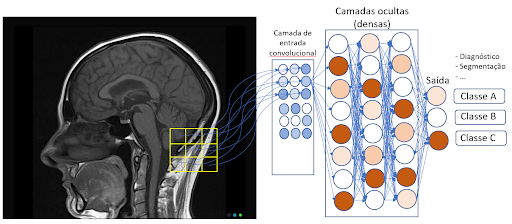
\includegraphics[width=.9\textwidth]{image1}
\caption{\label{fig1}Ilustração exemplificando uma possível arquitetura simples de uma rede profunda com uma camada de entrada convolucional (CNN – convolutional neural network), seguida por camadas ocultas densas ou completamente conectadas, e camada de saída com múltiplas classes. Nesta rede multicamadas estruturada espacialmente, assim como a imagem, o peso de cada nó (peso sináptico) é ajustado durante o processo de treinamento ou otimização da rede. As cores na ilustração representam as atividades em cada nó da rede em um determinado instante.}
\end{figure}

\section{Complexidade \texttt{LMC}}
Uma medida de complexidade estatística baseada em uma descrição probabilística de sistemas físicos e informacionais proposta por Lopez-Ruiz et. al. \cite{c39}, i.e., a chamada complexidade \texttt{LMC}, incorpora as principais características da noção intuitiva de tal medida para a qualidade de uma rede, ou da sua auto-organização, como uma grandeza que se contrapõe simultaneamente aos conceitos de ordem e aleatoriedade. Pode ser aplicado a muitas situações físicas e informacional a diferentes descrições de determinados sistemas. Além disso, o cálculo do seu valor não requer esforço computacional em muitos casos de interesse físico e computacional, sendo descrita como o produto da entropia informacional de Shannon pela distância do equilíbrio.

Nos fundamentos mais básicos, um objeto, procedimento ou sistema é dito complexo quando não corresponde a padrões considerados simples. Isso soa como um oxímoro, mas o conhecimento comum nos diz o que é simples e complexo: sistemas simplificados ou idealizações são sempre um ponto de partida para resolver problemas científicos. A noção de “complexidade” na física \cite{c7, c8} começa por considerar o cristal perfeito e o gás ideal isolado como exemplos de modelos simples e, portanto, como sistemas com “complexidade” zero. Recordemos brevemente suas principais características com “ordem”, “informação” e “equilíbrio”.

Uma estrutura cristalina perfeita é completamente ordenada e os seus componentes são organizados seguindo regras rigorosas de simetria. A distribuição de probabilidade para os estados possíveis desta estrutura é centrada em torno de um estado predominante de simetria perfeita. Uma pequena “informação” é suficiente para descrever a estrutura cristalina perfeita: as distâncias e as simetrias que definem sua célula elementar. As “informações” armazenadas neste sistema podem ser consideradas mínimas. Por outro lado, um sistema em caos completo isolado é completamente desordenado. O sistema pode ser encontrado em qualquer um de seus estados possíveis com a mesma probabilidade. Todos eles contribuem em igual medida para a “informação” armazenada no sistema. Tem, portanto, um máximo de “informação”. Esses dois sistemas simples são extremos na escala de “ordem” e “informação”. Segue-se que a definição de “complexidade” não deve ser feita apenas em termos de “ordem” ou “informação”.

\begin{figure}
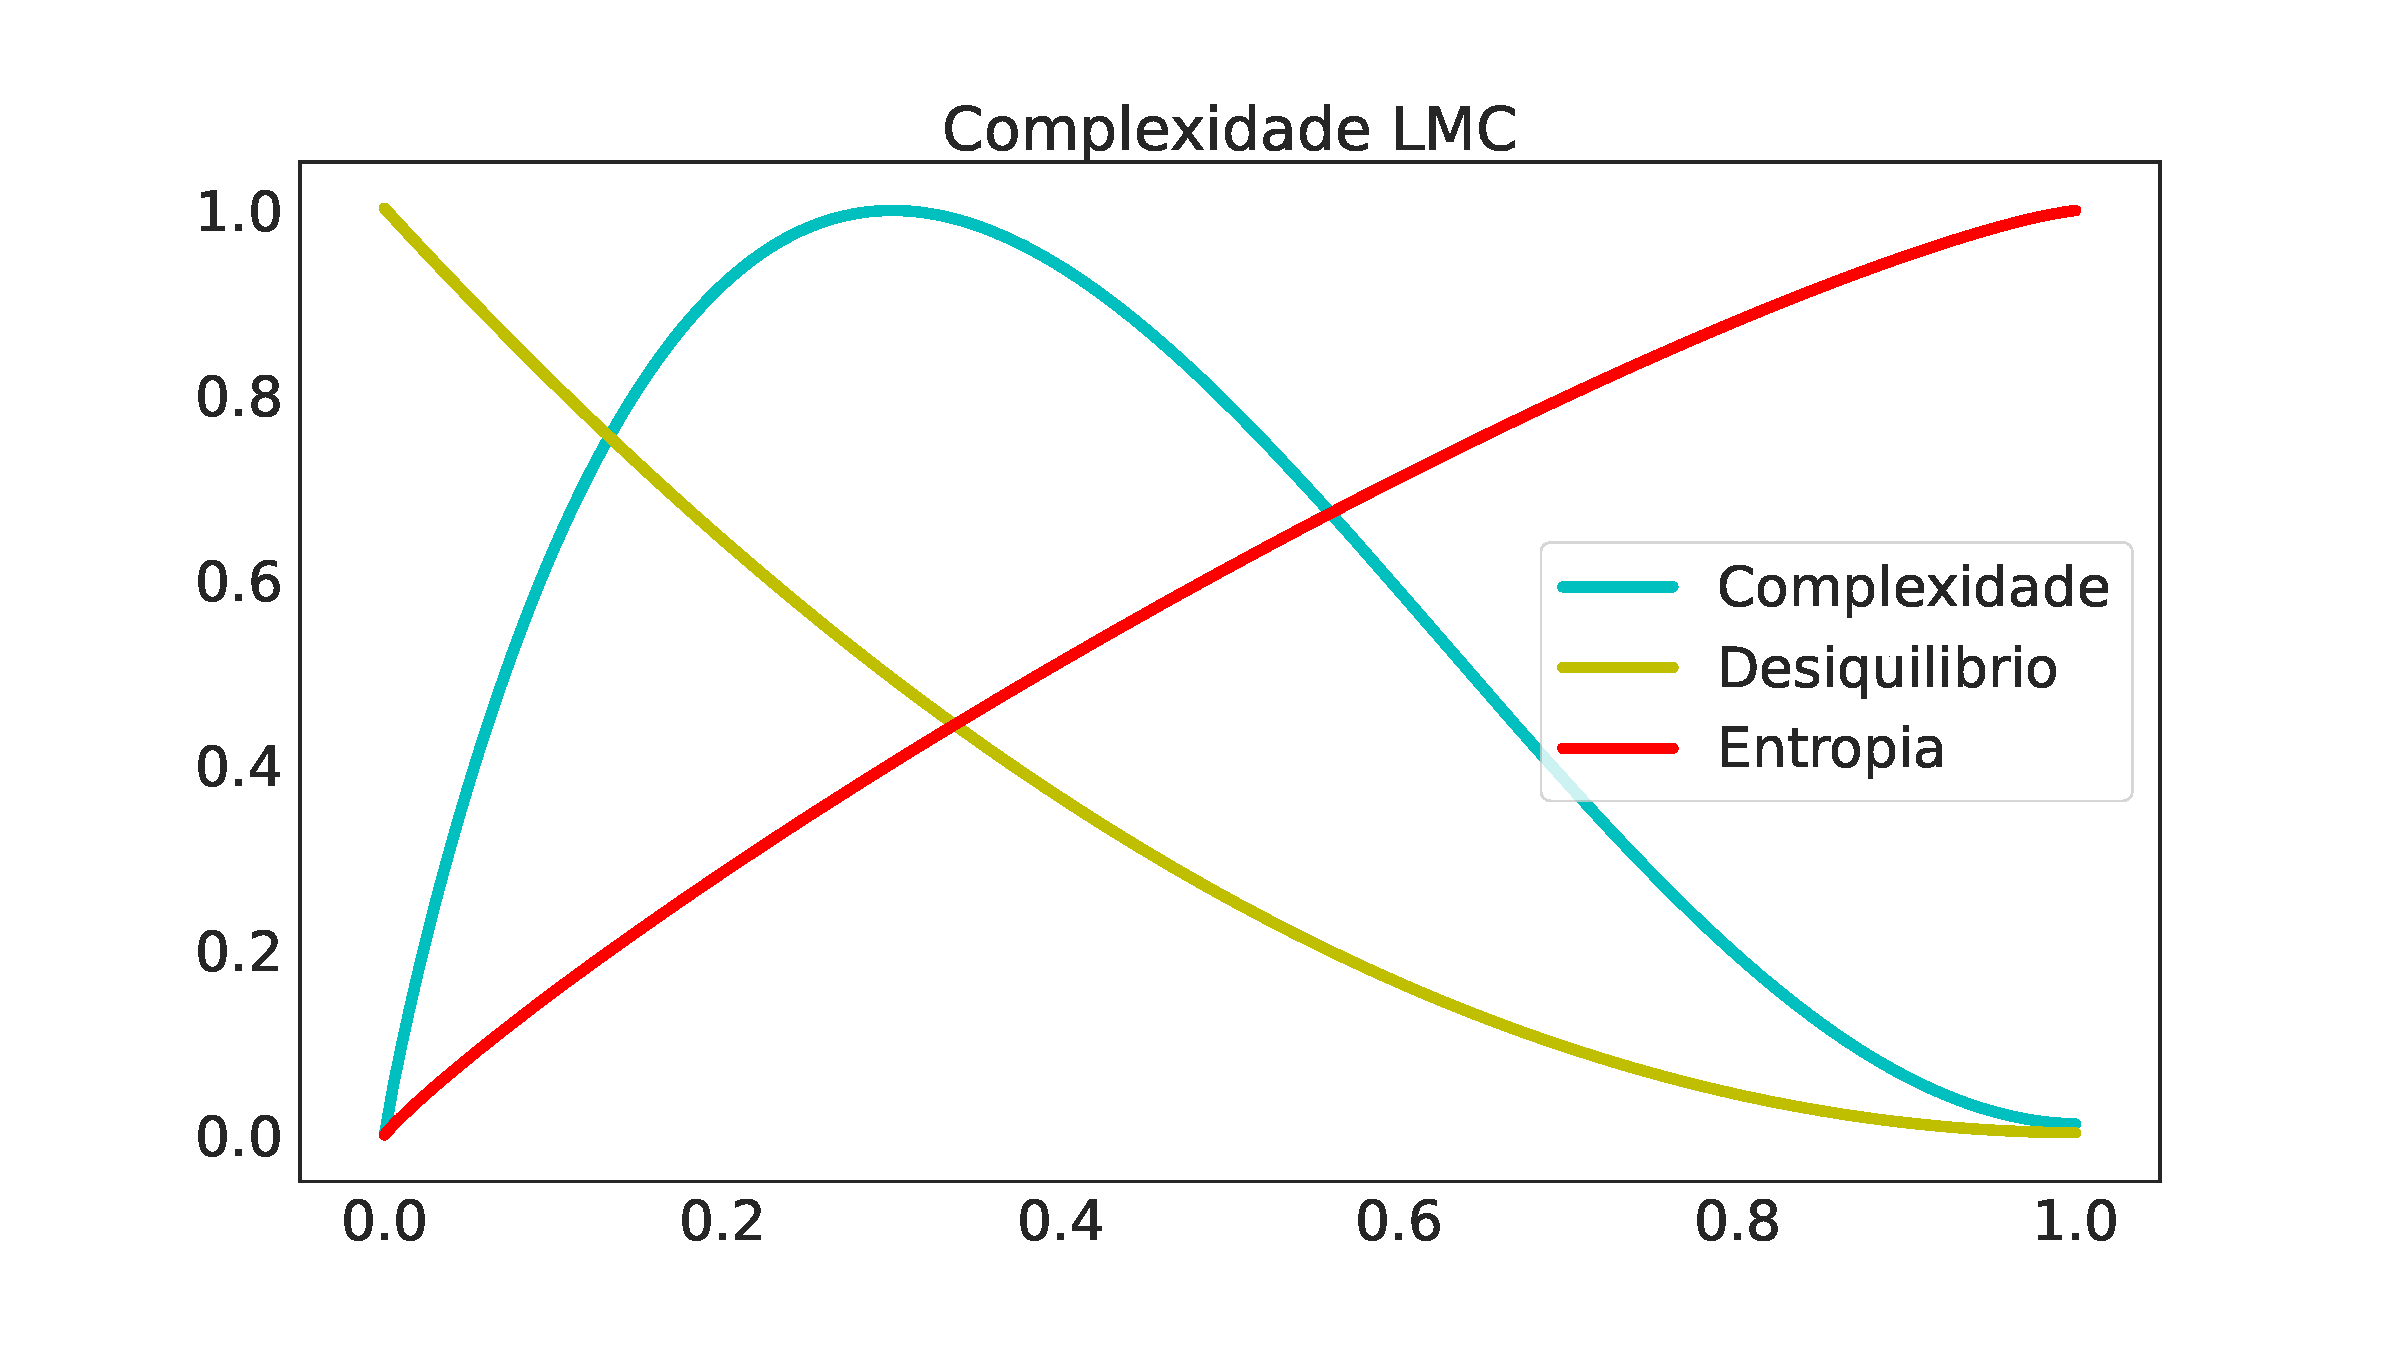
\includegraphics[width=.9\textwidth]{lmc}
\caption{\label{fig2}Ilustração mostrando a ideia por trás do conceito de complexidade \texttt{LMC}. O gráfico mostra três grandezas: a entropia informacional ou informação (entropia de Shannon), a distância do equilíbrio ou desequilíbrio, e a complexidade como o produto entre informação e desequilíbrio. Tanto na situação de ordem completa como no caos completo, i.e., aleatoriedade absoluta, a complexidade é baixa, assim, a complexidade ocorre entre a ordem e o caos.}
\end{figure}


Pode parecer razoável propor uma medida de “complexidade” adotando algum tipo de distância da distribuição equiprovável dos estados acessíveis do sistema \cite{c4}. Definido dessa forma, “desequilíbrio” daria uma idéia da hierarquia probabilística do sistema. “Desequilíbrio” seria diferente de zero se houvesse estados privilegiados, ou mais prováveis, entre os acessíveis. Mas somente isso não funcionaria. Voltando aos dois exemplos com os quais começamos, vê-se facilmente que uma estrutura perfeita está longe de ser uma equidistribuição entre os estados acessíveis porque um deles é totalmente prevalecente e, portanto, o “desequilíbrio” seria máximo. Para caos completo, o “desequilíbrio” seria zero por construção. Portanto, tal distância ou “desequilíbrio” (uma medida de uma hierarquia probabilística) não pode ser diretamente associado à “complexidade”.

A informação de Shannon ou entropia H pode continuar a ser usada como uma magnitude numa situação geral com N estados possíveis:

\begin{equation}
H = -k \, \sum^N_{i=1} \, p_i  \; log \, p_i
\end{equation}

com $k$ como uma constante real positiva, e $p_i$ as probabilidades normalizadas associadas,
$\sum p_i = 1$. Um sistema isolado em equilíbrio apresenta equiprobabilidade, $p_i = \frac{1}{N}$ para todo $i$ dentro dos estados possíveis e esta é uma situação de máxima entropia.
\begin{equation}
H_{max} =  -k \, \sum^N_{i=1} \, \frac{1}{N}  \; log \, \frac{1}{N}  = -k \, N \, \frac{1}{N} \; log \, \frac{1}{N} = k \; log \, N
\end{equation}
Se o sistema está fora do equilíbrio, a entropia $H$ pode ser expandida em torno do seu máximo $H_{max}$:
\begin{equation}
\label{eq3}
H(p1,p2, \ldots , p_N) = k \; log \, N - \frac{NK}{2} \sum^N_{i=1} \; \left( p_i - \frac{1}{N} \right)^2 + \ldots = H_{max} - \frac{NK}{2}D + \ldots
\end{equation}
onde surge a quantidade $D = \sum^N_{i=1} \; \left( p_i - \frac{1}{N} \right)^2$, que chamamos de desequilíbrio, como um tipo de distância da configuração do equilíbrio. Se a equação (\ref{eq3}) for multiplicada por $H$, obtemos: 
\begin{equation}
H^2 = H \cdot H_{max} - \frac{NK}{2}HD + k^2 f(N,p_i)
\end{equation}
onde $f(N,p_i)$	é a entropia multiplicada pelo restante da expansão de Taylor, que apresenta a forma
$\frac{1}{N} \sum_i (N p_i - 1)^{m}$ com $m>2$. Se assumirmos $C=H \cdot D$,
\begin{equation}
C = cte \cdot H \cdot (H_{max} - H) + K \bar{f}(N,p_i)
\end{equation}
com $cte^{-1}= \frac{NK}{2}$ e $\bar{f} = 2\frac{f}{N}$. A ideia de distância do equilíbrio, i.e., desequilíbrio está claro se enxergamos que $D$ é apenas a distância real 
$D \approx (H_{max}-H)$ % TODO
para distâncias na vizinhança da equiprobabilidade. Em um sistema completamente caótico, temos $H \to H_{max}$ e $D \to 0$, então $C \to 0$. Ao contrário, em um sistema completamente ordenado, $H \to 0$ e $D \to 1$, mas também $C \to 0$. Esses dois sistemas são considerados exemplos clássicos de modelos simples e são extremos em uma escala de desordem ($H$) ou desequilíbrio ($D$), mas devem apresentar complexidade nula em uma medida hipotética de complexidade. Este último comportamento assintótico é verificado pela variável $C$ na Figura \ref{fig2}. No lado esquerdo da figura, temos a máxima distancia do equilíbrio ou desequilíbrio e entropia mínima ou zero, indicando ordem ou previsibilidade completa, e, portanto, baixa complexidade. À medida que o sistema caminha para o equilíbrio o sistema pode passar por estágio de auto-organização, com aumento da entropia e redução do desequilíbrio, construindo estados de alta complexidade. Por outro lado, caminhando para o equilíbrio total (desequilíbrio zero) do sistema, a desordem ou entropia atinge seu patamar máximo, tornando-se totalmente imprevisível, e, portanto, complexidade zero.

\section{Complexidade \texttt{SampEn\textsubscript{2D}}}
Outro meio de avaliar a complexidade a ser considerada neste projeto é a entropia amostral (\texttt{SampEn\textsubscript{2D}}) estimada em diferentes escalas (\texttt{MSE}). A \texttt{SampEn\textsubscript{2D}} foi definida como uma extensão da \texttt{SampEn} unidimensional e tem como objetivo de medir o nível de irregularidade de padrões de pesos. Brevemente, o algoritmo da \texttt{SampEn\textsubscript{2D}} computa a possibilidade que padrões similares de tamanho $m$ continuarão similares para tamanhos $m+1$. Configurando a \texttt{SampEn\textsubscript{2D}}, o tamanho de padrões ($m$), bem como um fator de tolerância ($r$) é necessário para comparar a similaridade entre dois padrões, o último refletindo como restringir pesos dentro dos padrões são considerados similares. Quanto mais alto o valor de $r$, mais flexível será o critério de similaridade e mais padrões similares serão encontrados pela \texttt{SampEn\textsubscript{2D}}.

Seja $u(i, j)$ o conjunto de pesos em uma camada da rede DL estruturada em duas dimensões com largura $W$ e altura $H$ e $x_m (a, b)$ o subconjunto de pesos de u dentro do intervalo de $(a,b)$ até $(a + m-1, b + m-1)$. Em outras palavras, $x_m (a, b)$ é uma janela quadrada de pesos de $u$ com origem em $(a,b)$. As Equações de (\ref{eq6}) a (\ref{eq10}) definem a \texttt{SampEn\textsubscript{2D}}

\begin{equation}
\label{eq6}
SampEn_{2D}(u, m, r) = - ln \frac{U^{m+1}(r)}{U^m(r)}
\end{equation}

\begin{equation}
\label{eq7}
U^m(r) = \frac{1}{N_m}\sum U^m_{i,j}
\end{equation}

\begin{equation}
\label{eq8}
U^m_{i,j} = \frac{\text{\# of }x_m(a,b) \; | \; d[x_m(i,j), x_m(a,b) ] \leq r   }{N_m - 1}
\end{equation}

\begin{equation}
\label{eq9}
U^{m+1}(r) = \frac{1}{N_m} \sum U^{m+1}_{i,j}
\end{equation}

\begin{equation}
\label{eq10}
U^{m+1}_{i,j} = \frac{\text{\# of }x_{m+1}(a,b) \; | \; d[x_{m+1}(i,j), x_{m+1}(a,b) ] \leq r   }{N_{m+1} - 1}
\end{equation}

onde $a$ vai de $1$ a $H-m$, $b$ vai de $1$ a $W-m$ e $(a, b) \neq (i, j)$. $N_m$ é o número de padrões (janelas quadradas) que pode ser criada na estrutura de pesos $u$, para ambos os tamanhos $m$ e $m+1$. A função distância $d[\cdot]$ é definida na Equação (\ref{eq11}).
\begin{equation}
\label{eq11}
d[x_m(i,j), x_m(a,b)] = max(|u(i+k, j+k) - u(a+k, b+l)|)
\end{equation}

Já a MSE\textsubscript{2D} envolve a subamostragem em diferentes escalas dos sinais temporais e espaciais. A este padrão subamostrado aplica-se o algoritmo de \texttt{SampEn\textsubscript{2D}} considerando um intervalo de escala tipicamente de 1 a 20. Com o comportamento da \texttt{SampEn\textsubscript{2D}} em diferentes escalas se tem uma melhor ideia do tipo de processo que gerou aquele padrão, i.e., um processo estocástico, um processo que gere auto-similaridades em diferentes escalas (objetos fractais), processos oscilatórios regulares, entre outros.

\section{Repositórios de Imagens Médicas}
\label{sec:repositorios}
Com o objetivo de acessar diferentes modalidades de imagens de diferentes regiões do corpo, serão considerados repositórios públicos de imagens médicas como os detalhados abaixo. A utilização de repositórios públicos favorece também a necessária reprodutibilidade dos estudos, o que é importante em trabalhos acadêmicos.

\begin{itemize}
\item A coleção de imagens \texttt{MedMNIST v2} \cite{Yang2021}, contendo 12 datasets de imagens 2D e 6 datasets 3D, com um total de 708.069 imagens 2D e 10.214 imagens 3D, rotuladas para um conjunto diverso de modalidades biomédicas. Este conjunto contém um Benchmark de referência e códigos para reproduzir os resultados do artigo de referência.

\item O arquivo de imagens de radiologia de raios-X torácicos do instituto norte americano de saúde (National Institutes of Health – NIH) que contém 100.000 imagens, dados clínicos associados, anotações, e diagnósticos \cite{c40}; 
\item O arquivo de imagens de cânceres (The Cancer Imaging Archive – TCIA) também do NIH \cite{c41}, com imagens do consórcio de dados pulmonares LIDC (do inglês, \textit{Lung Image Database Consortium}), banco de dados de imagens de referência para avaliar a resposta à terapia de câncer de pulmão (RIDER) \cite{c42}, imagens de ressonância magnética (MRI) de mama, tomografias de emissões de pósitrons (PET) / tomografias computadorizadas (CT) pulmonares, neuroimagens MRI cerebrais, colonografia CT, colonoscopia virtual (CV).
\item A série de estudos de imagens de acesso aberto OASIS (do inglês, \textit{Open Access Series of Imaging Studies}) \cite{c43} é um repositório que armazena conjuntos de dados de neuroimagem do cérebro disponíveis livremente para a comunidade científica, com 1098 indivíduos, 2168 exames de MRIs, 1608 exames de PET. 
\end{itemize}

\section{Métodos de avaliação}
\label{sec:metodos}

Para avaliar a complexidade, sua evolução e impacto em relação as redes neurais é necessário definir uma metodologia tanto sobre como será feita a medição da complexidade, quanto sobre quais redes e estruturas arquitetônicas serão avaliadas. Uma parte do cronograma será dedicada para estabelecer melhor os três critérios definidos abaixo:

\begin{enumerate}
\item[Datasets] Criação de um conjunto de problemas a serem resolvidos com redes neurais, e.g., classificação e segmentação usando os repositórios da seção \ref{sec:repositorios}, que servirão como referência de uma aplicação prática completa, i.e., treinamento da rede com dados e posterior validação e inferência com outro conjunto de dados para estabelerecer a performance da rede.
\item[Redes] Definição das estruturas de rede a serem estudadas, com foco nos blocos principais, desde os módelos primitivos como blocos convolucionais e densos (\textit{fully connected}), até modulos de arquiteturas consagradas, e.g., módulo \texttt{Inception} \cite{c11}, módulo \texttt{Residual learning} \cite{c12}, \texttt{self-attention} \cite{Vaswani2017}. Como também efeitos em partes separadas das redes, e.g., comparar as partes de contração e expansão de uma U-Net \cite{c9}, comparar a complexidade na parte convolucional e densa de uma rede como AlexNet \cite{c4}
\item[Métricas] Definição das implementações das métricas de complexidade usadas, e.g., \texttt{LMC} e \texttt{SampEn}, junto com os meta-parâmetros de cada uma, e.g., número de bins nos histogramas ou definição da função de probabilidade que define o desequilíbrio da \texttt{LMC}, tamanho da janela utilizada na \texttt{SampEn}.
\end{enumerate}


\chapter{Resultados preliminares \texttt{LMC}}
\begin{figure}
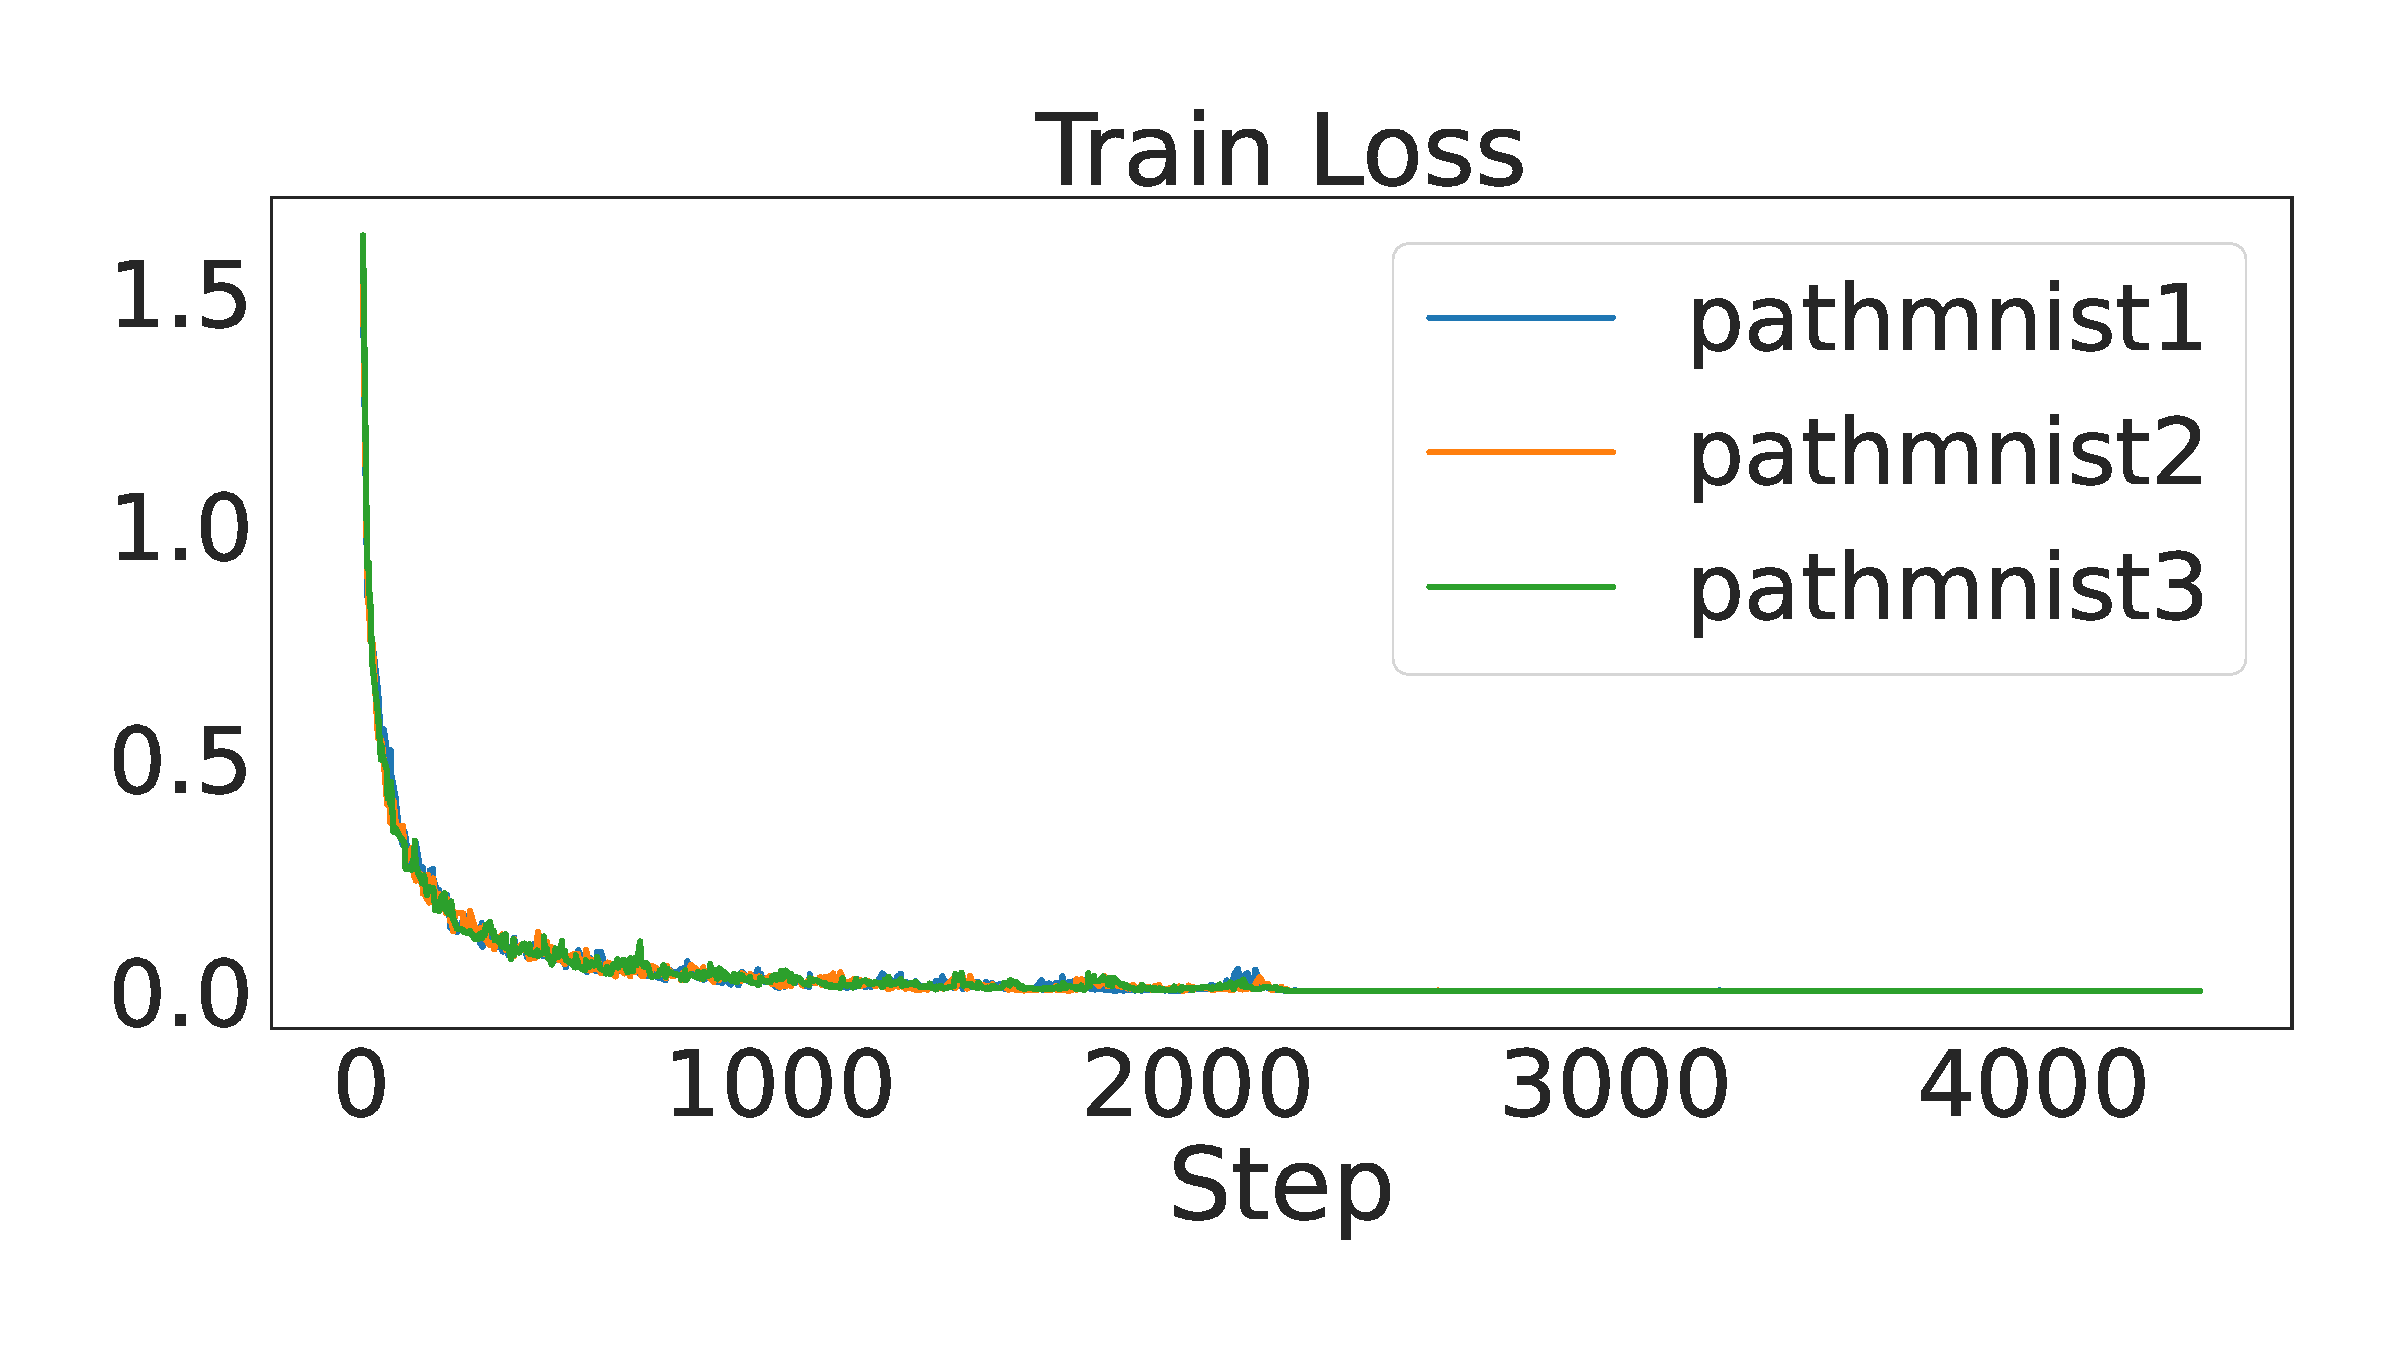
\includegraphics[width=.5\textwidth]{preliminar/fapesp-loss}%
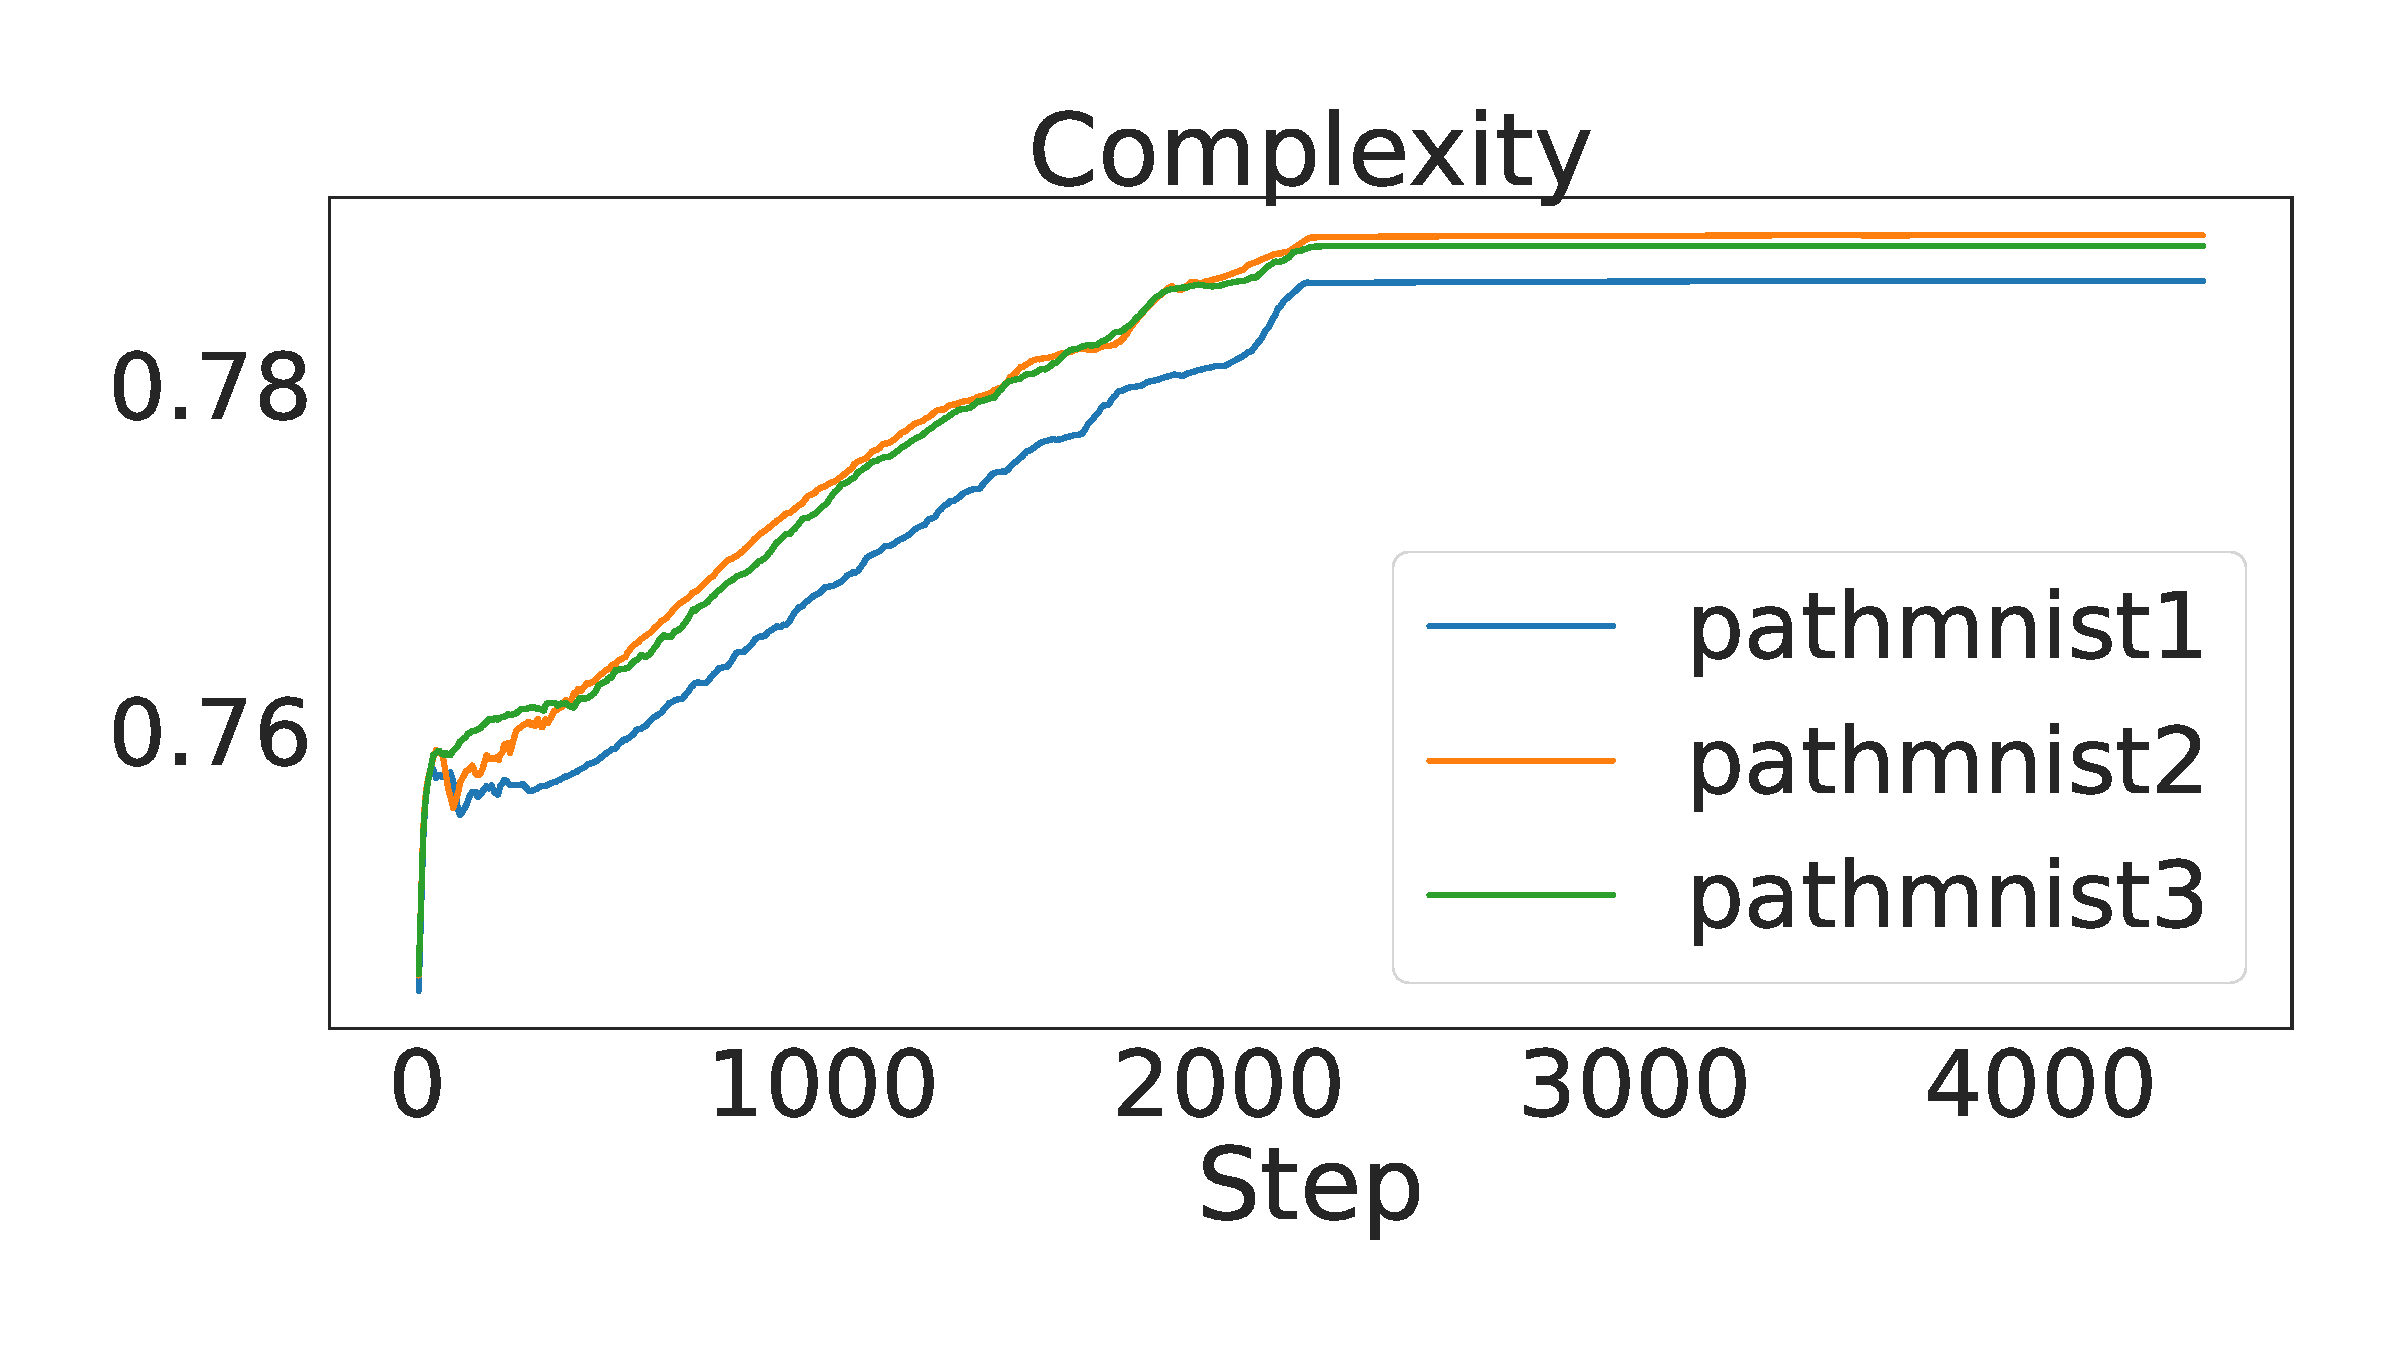
\includegraphics[width=.5\textwidth]{preliminar/fapesp-complexity}\\
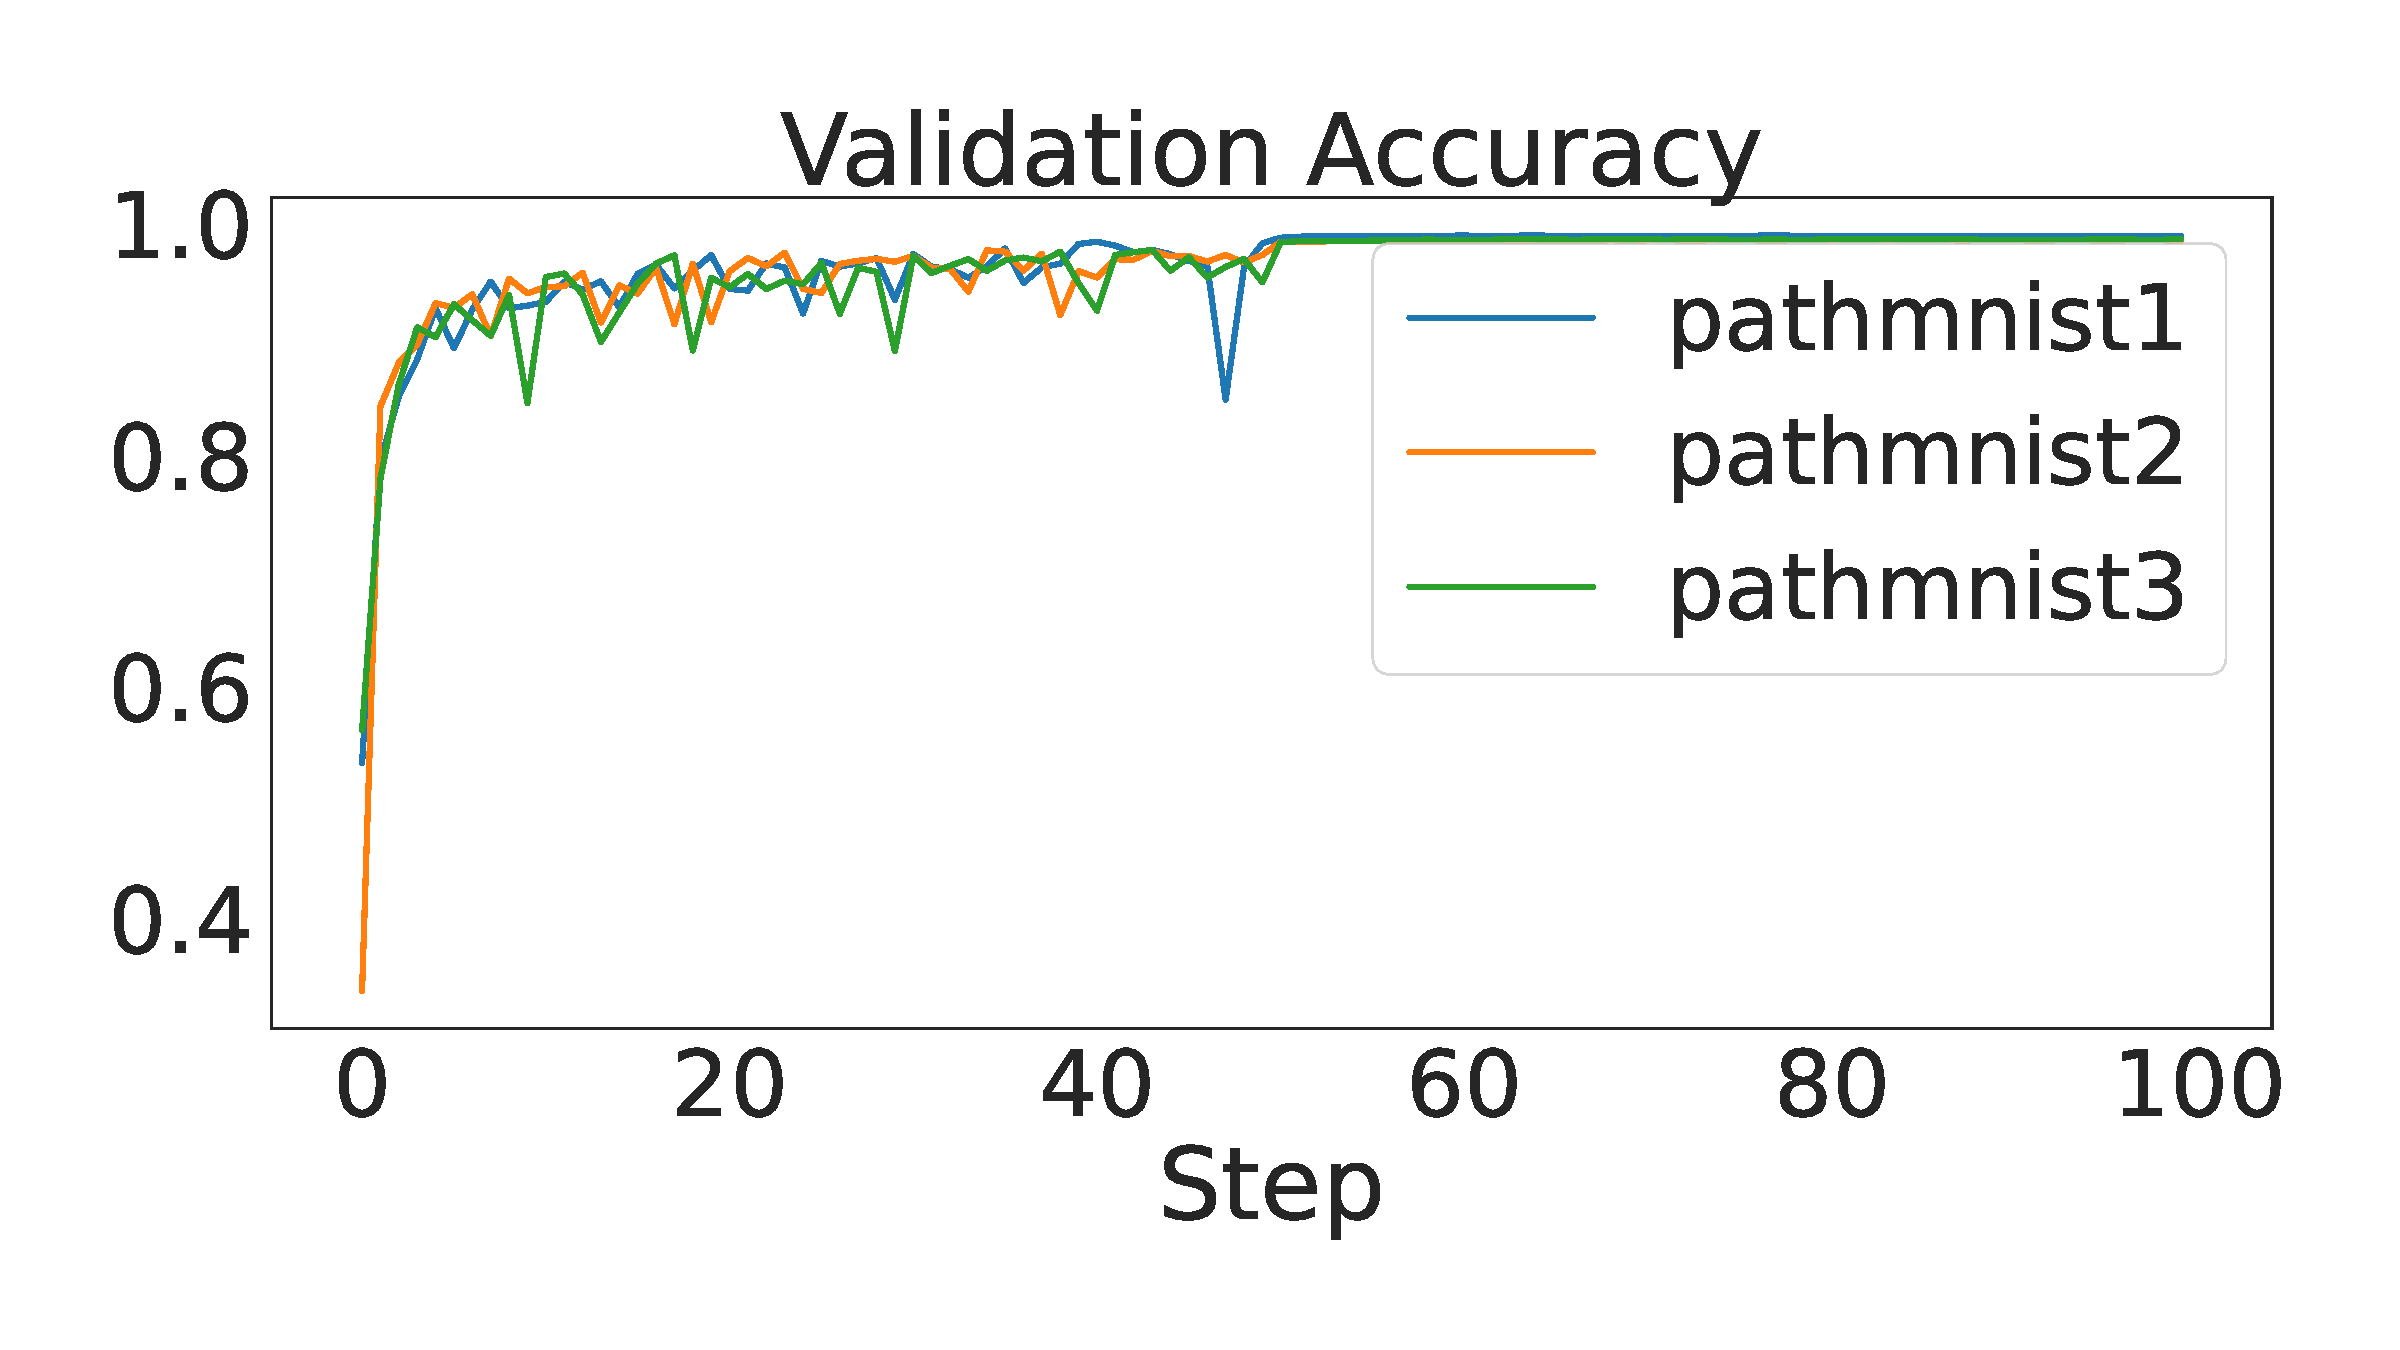
\includegraphics[width=.5\textwidth]{preliminar/fapesp-val_accuracy}%
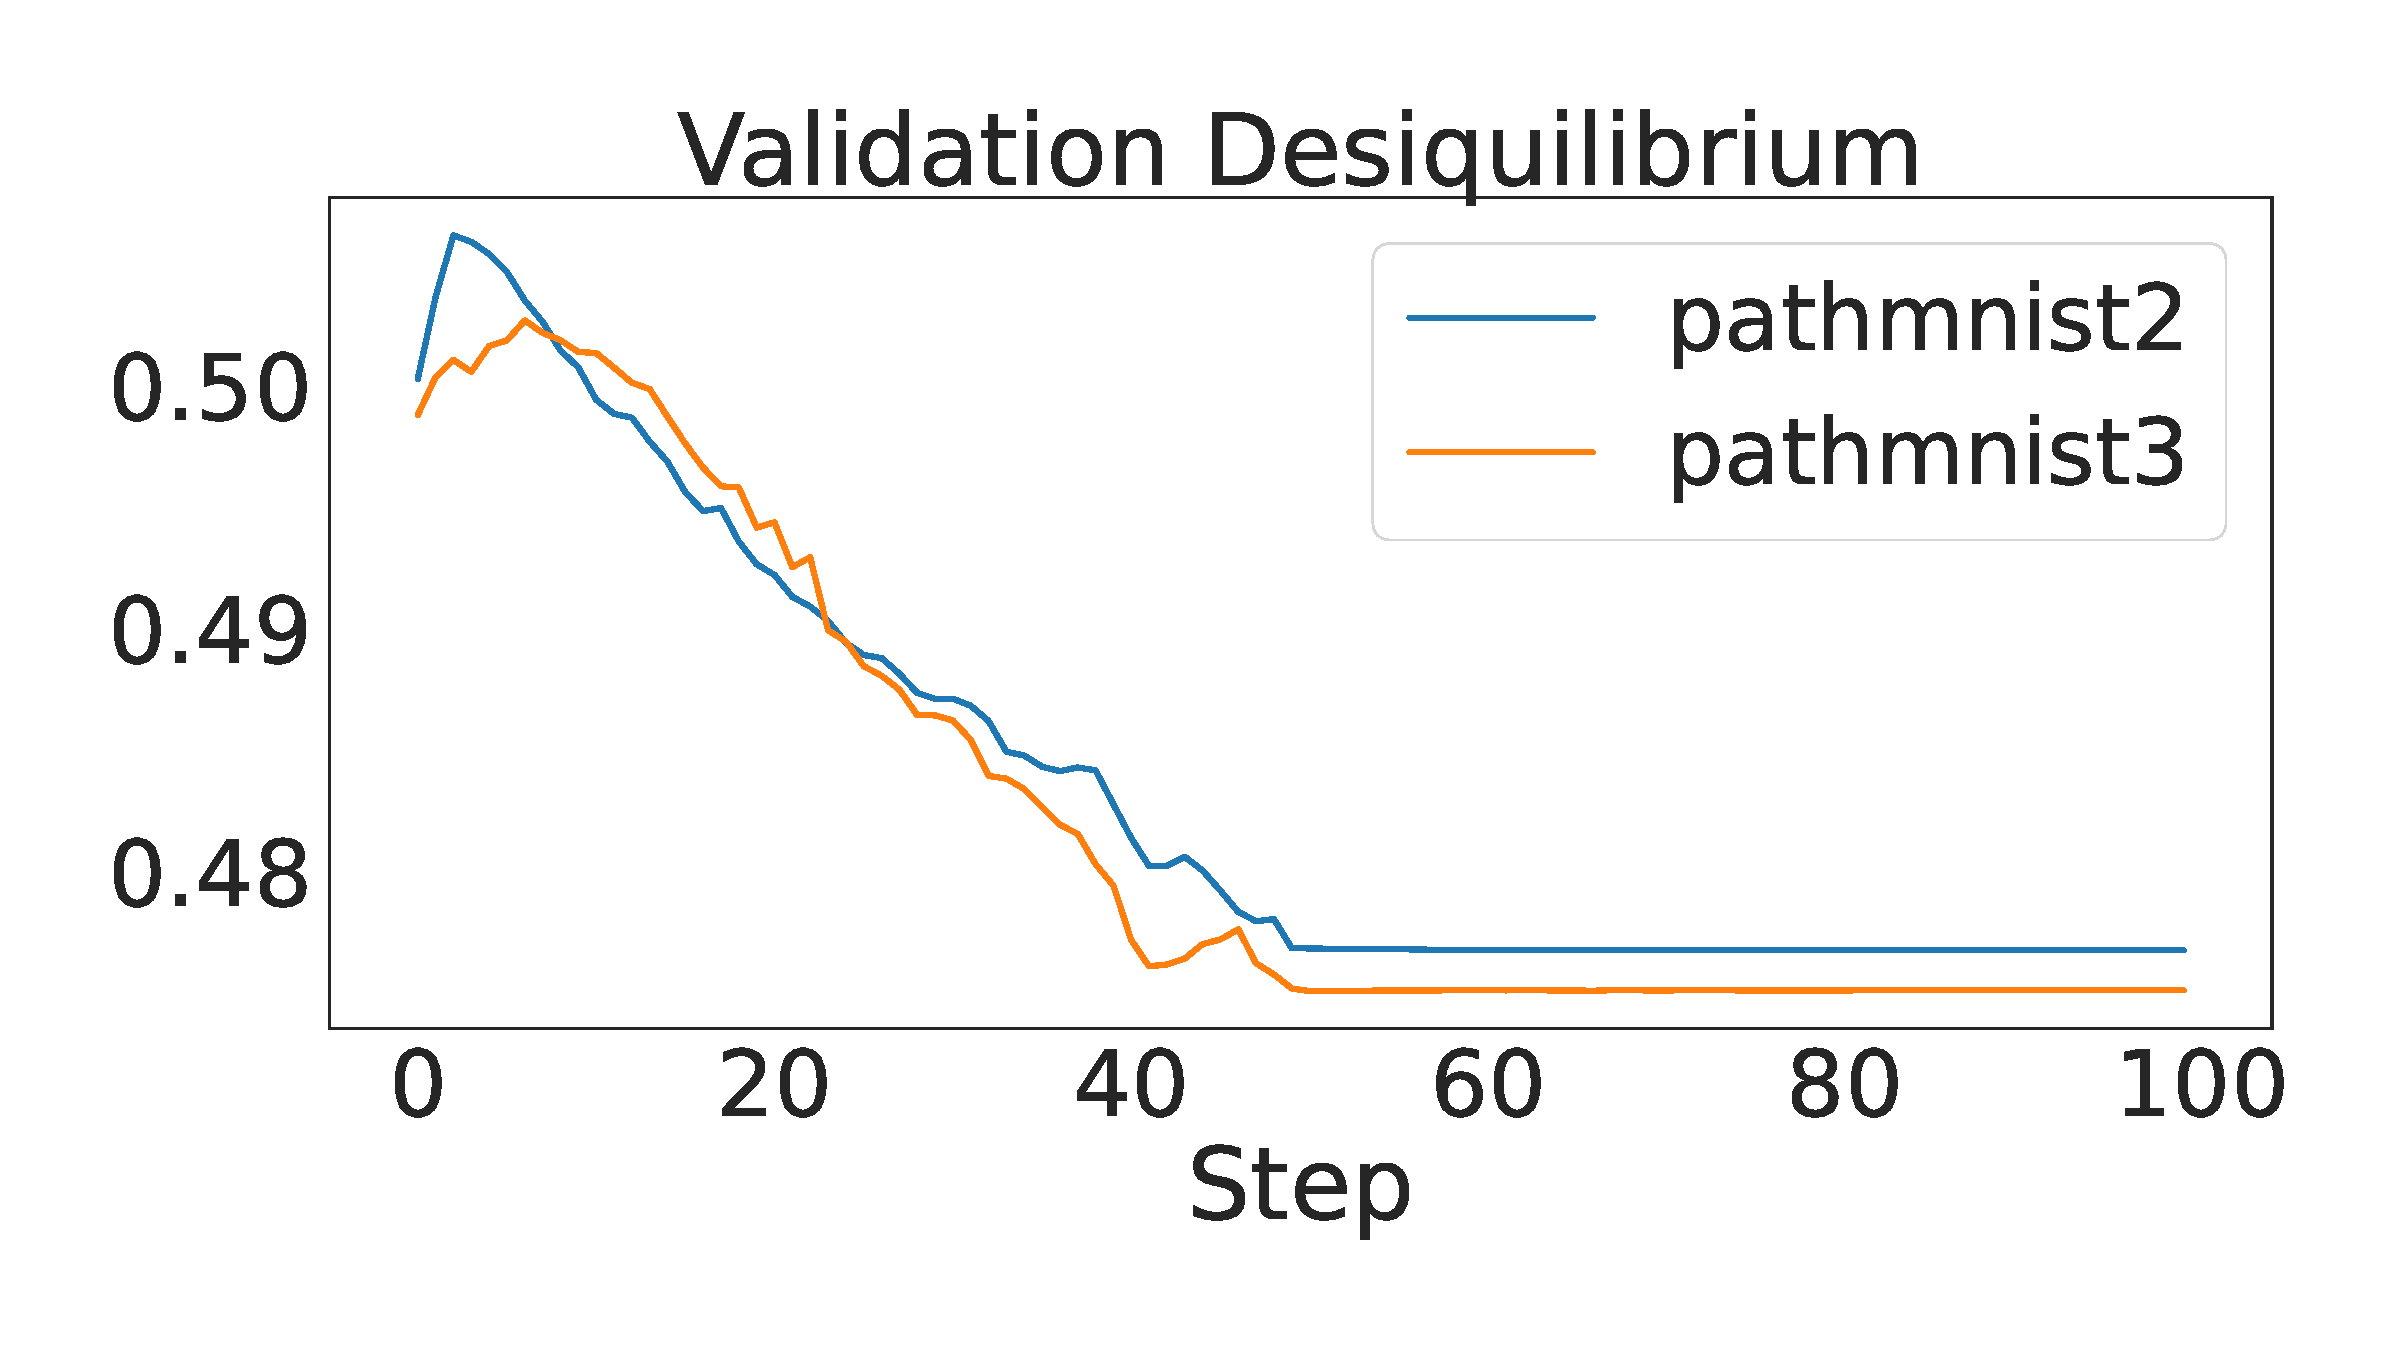
\includegraphics[width=.5\textwidth]{preliminar/fapesp-val_desiquilibrium}\\
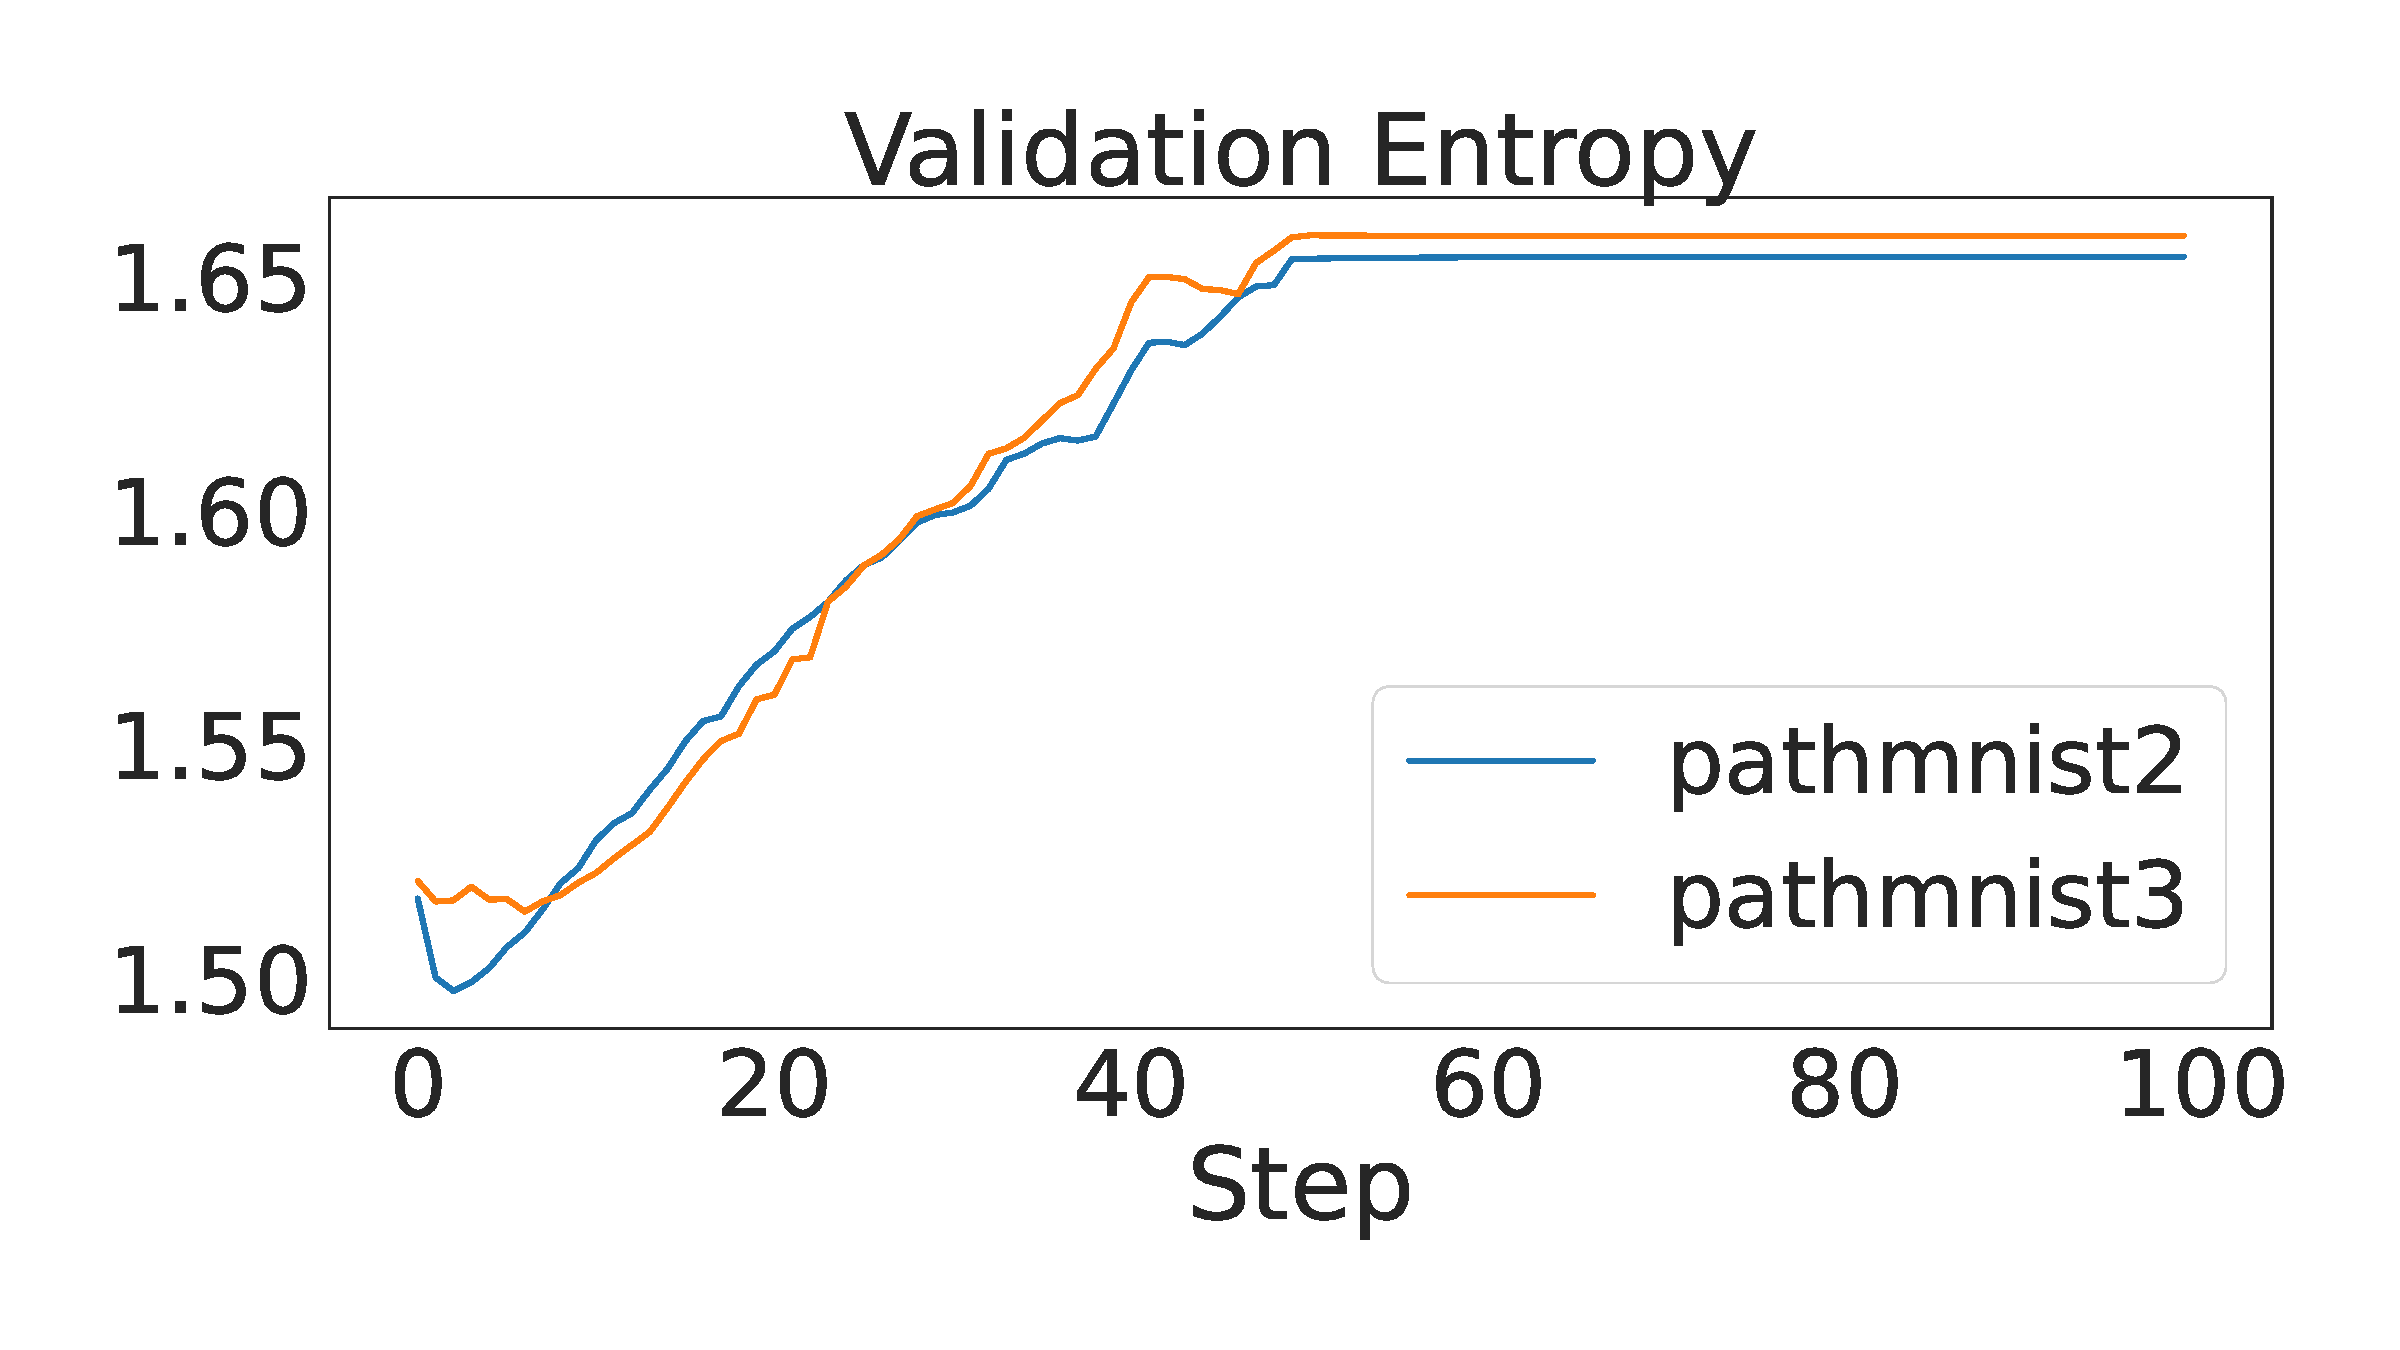
\includegraphics[width=.5\textwidth]{preliminar/fapesp-val_entropy}%
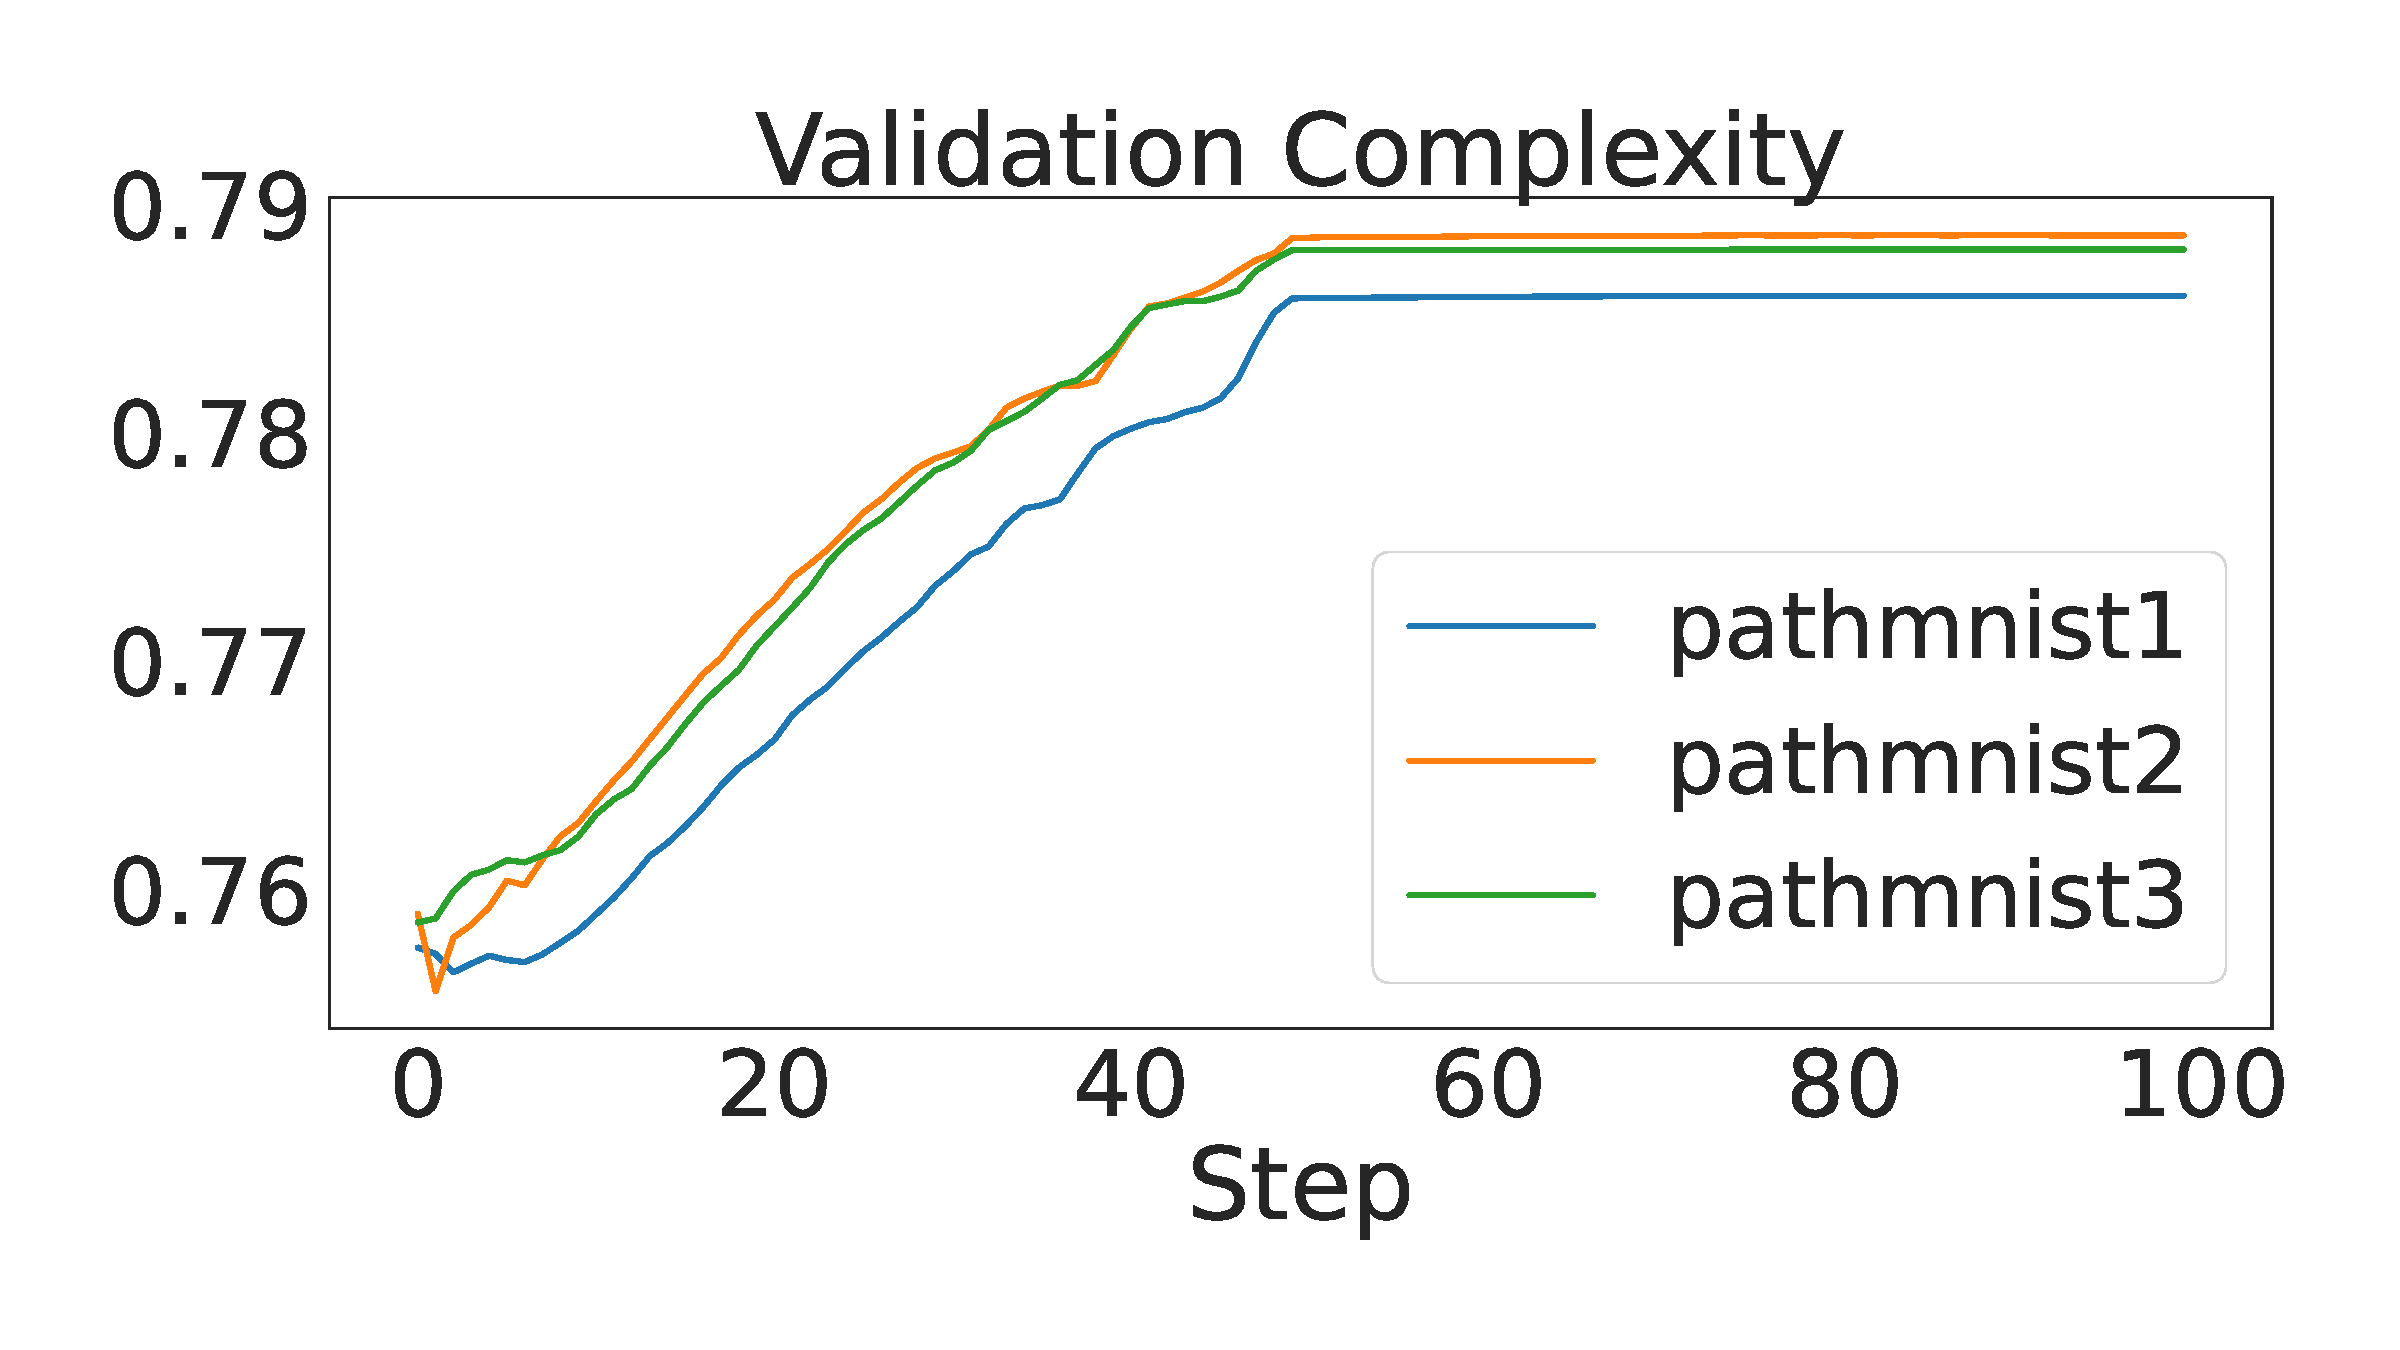
\includegraphics[width=.5\textwidth]{preliminar/fapesp-val_complexity}\\

\caption{\label{fig3}Gráficos com resultados preliminares com experimento em classificação de imagens do dataset PathMNIST do conjunto MedMNISTv2 \cite{MEDMNIST}. Na linha superior estão os gráficos de todas as iterações, mostrando a perda (\textit{Train Loss}) e a complexidade (\textit{Complexity}). As duas linhas inferiores são gráficos por época usando o conjunto de validação, mostrando a acurácia (\textit{Accuracy}), desiquilíbrio (\textit{Desiquilibrium}), entropia (\textit{Entropy}) e a complexidade (\textit{Complexity}). Os gráficos da complexidade (direita na linha superior e central) indicam que a evolução é de crescimento durante o treinamento. }
\end{figure}

A Figura \ref{fig3} mostra a evolução da complexidade \texttt{LMC} e as suas componentes, i.e., desequilíbrio e entropia. O comportamento da complexidade durante o treinamento indica que a rede se auto-organiza em termos do seu padrão de pesos para resolver o problema de classificação das imagens. Lembrando que esta dinâmica é conduzida pelos algoritmos de otimização e dirigida pela função de perda. Estes resultados sugerem que a função de complexidade pode ajudar a função de perda na otimização da rede.

Os resultados foram feitos utilizando os scripts usados pelos autores do dataset \texttt{MedMNISTv2}, que podem ser encontrados em \url{https://github.com/MedMNIST/experiments/tree/main/MedMNIST2D}, alterando apenas para exportar os logs para o \texttt{TensorBoard} e com uma implementação simples da entropia \texttt{LMC}.

Nos estudos preliminares alguns desafios a serem estudados já foram encontrados, como a definição do que é o estado de equilíbrio das redes neurais, já que as camadas podem ser inicializadas de várias formas, e.g., distribuições lineares, normais, e inicialização Xavier \cite{Glorot2010}.

Outro desafio é sobre a quantidade de \textit{bins} utilizados no cálculo do histograma que altera bastante a resposta das funções de desiquilíbrio e entropia.

\chapter{Resultados Esperados}
O presente projeto irá contribuir para entender o comportamento das chamadas redes de aprendizado profundo quando aplicada a imagens médicas quanto ao seu poder de auto-organização de padrões de pesos sinápticos. O método proposto poderá ser usado como critério para a escolha das melhores arquiteturas de redes DL e métodos de treinamento para variadas aplicações em imagens médicas. A referida avaliação em diferentes contextos e modalidades de imagens médicas levará às melhores arquiteturas de redes para as diferentes aplicações no âmbito de imagens médicas. Portanto, pode vislumbrar a produção de artigos em revistas relevante para a especialidade e patente sobre o método. Pode-se prever também a formação de doutores e mestres na especialidade de inteligência artificial em imagens médicas.

Espera-se que ao término da pesquisa seja possível treinar redes com um foco maior em desenvolver a complexidade, e não somente na redução do erro do treinamento. Isto pode levar, caso a hipótese seja válida, a redes mais eficientes e precisas, além de reduzir os recursos, e.g., o tempo, usados no treinamento das redes.

Cabe notar que o impacto desta pesquisa não fica restrito somente ao contexto de imagens médicas. Qualquer rede artificial usada em IA poderá beneficiar destes resultados, de forma maior ou menor, de acordo com sua arquitetura interna e como a complexidade afeta sua performance.

\chapter{Cronograma}
O projeto pode ser dividido em duas etapas, a saber, demonstração de validade das medidas de complexidade com índice de qualidade das redes DL; e dos seus treinamentos e aplicação e validação do índice de qualidade em diferentes contextos de arquiteturas, modalidade de imagens médicas, e finalidades de aplicações. 

A primeira etapa é mais extensa e servirá como base para a segunda etapa como também para estudos futuros, fornecendo as evidências ciêntificas sobre a relação da Complexidade com a performance e treinamento da rede. Além da criação de uma infraestrutura facilitando e automatizando os testes e processamento dos resultados, e.g., criação de tabelas e gráficos sintetizando os resultados. Isto facilitará entender o impacto de cada mudança, seja na arquitetura ou na implementação do código, na performance final da rede, que é o que importa para o público final, i.e., comunidade médica.
 
Na primeira etapa também será definido um \textit{Benchmark}, com os melhores resultados possíveis com as tecnologias atuais, apenas observando a Complexidade. Na segunda etapa o objetivo será utilizar a Complexidade para melhorar as redes e superar os resultados do \textit{Benchmark}.

Cabe ressaltar que durante todo o tempo serão enviados para publicação os resultados da primeira e segunda etapa, bem como os resultados secundários provenientes da aplicação das redes DL em diferentes contextos, as tarefas de escrita dos resultados, relatórios e manuscritos estão implícitas em cada tarefa.

A organização temporal do projeto segundo o exposto na Figura \ref{figcronograma}, utilizando os ítens definidos abaixo:

\textbf{Infraestrutura:}
\begin{description}
\item[Datasets] Definir os datasets a serem utilizados durante o estudo, com vários problemas diferentes, e.g., classificação e segmentação, como a aquisição dos mesmos, incluindo processos burocráticos que forem necessários para o uso de cada dataset, e.g., conformidade com as necessidades éticas de cada dataset.
\item[Redes] Definir as redes a serem utilizadas, abrangendo o maior número de blocos básicos apresentados na seção \ref{sec:metodos}, sem se restringir a estes já que podem existir outras arquiteturas interessantes de serem estudadas, definindo também seções da rede que devam ser estudadas separadamente.
\item[Benchmark] Estabelecer resultados base entre as Redes e Datasets, tentando replicar os resultados da literatura, quando disponíveis, e estabelecer a melhor rede para cada tipo de problema, assim como suas medidas de performance como acurácia.
\item[Métricas] Implementar o código-fonte de cada métrica a ser utilizada, testando as mesmas em um subconjunto de Datasets e Redes, ajustado para ter uma variedade de dados e usar poucos recursos nesta fase. Adequando os meta-parâmetros de cada métrica como também resolvendo os detalhes da implementação numérica de cada uma no contexto de redes neurais e do framework utilizado (\texttt{PyTorch} ou \texttt{TensorFlow}).
\item[Re-Avaliação] Re-avaliar as escolhas feitas anteriormente, já com os resultados adquiridos nos primeiros trimestres, incluindo novos elementos que considerarmos interessantes estudar, e.g., novas arquiteturas e conjuntos de dados. Também pode ser uma oportunidade para alterar alguma implementação das métricas que se mostrem necessárias. 
\end{description}

\textbf{Validação da Complexidade:}
\begin{description}
\item[Escolha arquitetura] Avaliar, utilizando os dados coletados e conceitos aprendidos na etapa anterior, como a complexidade pode ajudar a escolher arquiteturas para os problemas. Arquitetura aqui não se restringe ao tipo principal de rede, e.g., \texttt{InceptionNet} ou \texttt{ResNET}, mas também, por exemplo, ao número de camadas e dimensões de cada camada.
\item[Treinamento] Avaliar como a Complexidade pode ser utilizada como uma informação adicional no treinamento das redes, em conjunto com a perda de treinamento que normalmente guia o processo de otimização das redes.
\end{description}

\textbf{Aplicações:}
\begin{description}
\item[Aplicações clínicas] Avaliar como a complexidade pode ser utilizada para analisar como uma rede profunda aprende com dados de imagens clínicas nas terefas de diagnóstico, segmentação, e corregistro. O objetivo aqui é Selecinoar algumas aplicações no contexto do  Hospital das Clínicas de Ribeirão Preto, como o diagnóstico e prognóstico de doenças degenerativas cerebrais.
\item[Suporte ao tratamento guiado por imagens (IGT)] Testar o método em alguns cenários de suporte ao tratamento, mensurando o ganho clínico para os pacientes.  
\end{description}


\begin{figure}

%
% A fairly complicated example from section 2.9 of the package
% documentation. This reproduces an example from Wikipedia:
% http://en.wikipedia.org/wiki/Gantt_chart
%
\definecolor{barblue}{RGB}{153,204,254}
\definecolor{groupblue}{RGB}{51,102,254}
\definecolor{linkred}{RGB}{165,0,33}
\renewcommand\sfdefault{phv}
\renewcommand\mddefault{mc}
\renewcommand\bfdefault{bc}
\setganttlinklabel{s-s}{START-TO-START}
\setganttlinklabel{f-s}{FINISH-TO-START}
\setganttlinklabel{f-f}{FINISH-TO-FINISH}
\sffamily
\begin{ganttchart}[
    canvas/.append style={fill=none, draw=black!5, line width=.75pt},
    hgrid style/.style={draw=black!5, line width=.75pt},
    vgrid={*1{draw=black!5, line width=.75pt}},
    today=0,
    today rule/.style={
      draw=black!64,
      dash pattern=on 3.5pt off 4.5pt,
      line width=1.5pt
    },
    today label font=\small\bfseries,
    title/.style={draw=none, fill=none},
    title label font=\bfseries\footnotesize,
    title label node/.append style={below=7pt},
    include title in canvas=false,
    bar label font=\mdseries\small\color{black!70},
    bar label node/.append style={left=2cm},
    bar/.append style={draw=none, fill=black!63},
    bar incomplete/.append style={fill=barblue},
    bar progress label font=\mdseries\footnotesize\color{black!70},
    group incomplete/.append style={fill=groupblue},
    group left shift=0,
    group right shift=0,
    group height=.5,
    group peaks tip position=0,
    group label node/.append style={left=1.6cm},
    group progress label font=\bfseries\small,
    link/.style={-latex, line width=1.5pt, linkred},
    link label font=\scriptsize\bfseries,
    link label node/.append style={below left=-2pt and 0pt},
    x unit=0.7cm
  ]{1}{8}
  \gantttitle[
    title label node/.append style={below left=7pt and -3pt}
  ]{BIMESTRE:\quad1}{1}
  \gantttitlelist{2,...,12}{1} \\
  \ganttgroup[progress=0]{Infraestrutura}{1}{6} \\
  \ganttbar[progress=0,inline=false]{Datasets}{1}{1}\\
  \ganttbar[progress=0,inline=false]{Redes}{1}{2}\\
  \ganttbar[progress=0,inline=false]{Benchmark}{3}{3}\\
  \ganttbar[progress=0,inline=false]{Métricas}{1}{4}\\
  \ganttbar[progress=0,inline=false]{Re-avaliação}{5}{6}\\
  \ganttgroup[progress=0]{Validação}{7}{8} \\
  \ganttbar[progress=0,inline=false]{Escolha arquitetura}{7}{7}\\
  \ganttbar[progress=0,inline=false]{Treinamento}{8}{8}\\
  \ganttgroup[progress=0]{Aplicações}{9}{12} \\
  \ganttbar[progress=0,inline=false]{Aplicações clínicas}{9}{11}\\
  \ganttbar[progress=0,inline=false]{Suporte ao IGT}{10}{12}\\

\end{ganttchart}
\caption{\label{figcronograma}Cronograma de execução do presente projeto, segundo organização
trimestral.}

\end{figure}

\chapter{Recursos Disponíveis}
O grupo de pesquisa Computação em Sinais e Imagens Médicas – CSIM, coordenado pelo pesquisador proponente, dispõe de sala com computadores pessoais e um servidor de alta performance em outra sala climatizada com recursos de redundância energética (nobreaks). O servidor de alta performance computacional do grupo dispõe de uma configuração adequada e poder computacional suficiente para a execução deste projeto, com dois processadores totalizando 64 núcleos CPU de processamento, 500 GBytes de memória RAM, GPU NVidia P5000 com 2460 núcleos de processamento, e 8 TBytes de armazenamento de disco.


% ---
% Finaliza a parte no bookmark do PDF
% para que se inicie o bookmark na raiz
% e adiciona espaço de parte no Sumário
% ---
\phantompart

% ---
% Conclusão
% ---
%\chapter*[Considerações finais]{Considerações finais}
%\addcontentsline{toc}{chapter}{Considerações finais}

%\lipsum[31-33]

% ----------------------------------------------------------
% ELEMENTOS PÓS-TEXTUAIS
% ----------------------------------------------------------
\postextual

% ----------------------------------------------------------
% Referências bibliográficas
% ----------------------------------------------------------
\addcontentsline{toc}{section}{Referências}
\bibliography{projeto}

% ----------------------------------------------------------
% Glossário
% ----------------------------------------------------------
%
% Consulte o manual da classe abntex2 para orientações sobre o glossário.
%
%\glossary

% ----------------------------------------------------------
% Apêndices
% ----------------------------------------------------------

% ---
% Inicia os apêndices
% ---
%\begin{apendicesenv}

% Imprime uma página indicando o início dos apêndices
%\partapendices

%\end{apendicesenv}
% ---


% ----------------------------------------------------------
% Anexos
% ----------------------------------------------------------

% ---
% Inicia os anexos
% ---
%\begin{anexosenv}

% Imprime uma página indicando o início dos anexos
%\partanexos

% ---
%\chapter{Morbi ultrices rutrum lorem.}
% ---
%\lipsum[30]

% ---
%\chapter{Cras non urna sed feugiat cum sociis natoque penatibus et magnis dis
%parturient montes nascetur ridiculus mus}
% ---

%\lipsum[31]

% ---
%\chapter{Fusce facilisis lacinia dui}
% ---

%\lipsum[32]

%\end{anexosenv}

%---------------------------------------------------------------------
% INDICE REMISSIVO
%---------------------------------------------------------------------

\phantompart

\printindex


\end{document}
